\chapter{Fundamentação Teórica}

Neste capítulo, abordaremos tópicos fundamentais relacionados à virtualização e aos serviços de computação em nuvem de forma geral, proporcionando uma compreensão mais aprofundada de como funciona tecnologias e de qual forma são utilizadas, essencial para entender como funciona o OpenStack internamente.


\section{Introdução a Virtualização}

Para começarmos a falar sobre a virtualização, precisamos entender o que ela é, para que serve e quais são suas aplicações práticas. A virtualização nada mais é do que a criação virtual de um serviço computacional sobre um hardware e um software reais~\citep{chirammal2016mastering}. Quando falamos de real e virtual, devemos entender que o real é o que está efetivamente executando na máquina principal, no computador raiz, enquanto o virtual será originado a partir dele, como um convidado dentro do software/hardware real. Por isso, podemos chamá-lo de `Serviço Computacional Convidado' \textit{(Guest Computing Service)} ou, como na maioria dos casos estamos lidando com sistemas operacionais, é comum chamá-los de `SO Convidado' \textit{(Guest OS)} ou até mesmo `VM Convidada' \textit{(Guest VM)}. A maneira como essa VM (Máquina Virtual) é hospedada dentro do software principal depende de como ela vai ser criada~\citep{chirammal2016mastering}, falaremos mais sobre criação de VMs.

 É fundamental entender as aplicações práticas da virtualização, já que utilizamos a todo momento. As aplicações de virtualização são diversas e abrangem diferentes aspectos da tecnologia. Vamos explorar algumas dessas aplicações como mencionadas por \cite{chirammal2016mastering}:

\begin{itemize}
  \item \textbf{Consolidação de servidores}: A virtualização permite consolidar servidores, economizando energia e espaço físico. Ao reduzir o número de servidores físicos, há também menos componentes de rede e racks, resultando em economia de recursos e maior utilização de hardware.

  \item \textbf{Isolamento de serviços}: A virtualização facilita o isolamento de serviços, evitando a necessidade de servidores dedicados para cada aplicação e reduzindo custos com melhor uso dos recursos disponíveis.

  \item \textbf{Provisionamento rápido de servidores}: Com virtualização, máquinas virtuais podem ser criadas rapidamente a partir de imagens ou snapshots, sem precisar configurar manualmente recursos físicos, agilizando o processo.

  \item \textbf{Recuperação de desastres}: A virtualização simplifica a recuperação de desastres, com snapshots atualizados que podem ser reimplantados rapidamente. Técnicas de migração de VMs aumentam a flexibilidade nesse processo.

  \item \textbf{Balanceamento dinâmico de carga}: A virtualização permite mover VMs sobrecarregadas para servidores subutilizados, de acordo com políticas estabelecidas, otimizando o uso dos recursos.

  \item \textbf{Ambiente de desenvolvimento e teste mais rápido}: A virtualização facilita a criação de ambientes de teste temporários de forma rápida e segura, com a possibilidade de restaurar rapidamente imagens em caso de problemas.

  \item \textbf{Maior confiabilidade e segurança}: A virtualização cria uma camada de abstração que protege o sistema contra falhas físicas e permite configurar ambientes isolados, aumentando a segurança da infraestrutura.

  \item \textbf{Independência do hardware}: A virtualização elimina o lock-in de hardware, permitindo mais flexibilidade na escolha de equipamentos e garantindo maior continuidade operacional.
\end{itemize}


\subsection{Anéis de segurança na arquitetura x86\_64}
Neste projeto, vamos focar na orquestração de VMs com a arquitetura x86-64, que é a mais utilizada no mercado entre os diferentes serviços nuvem \citep{DataCenterCPUMarketAMDSurpassesIntelinShareGrowth}. Essa arquitetura apresenta uma forma interessante de segurança, separando as aplicações em anéis de segurança. Ao todo, temos quatro anéis, sendo o anel 0 o mais privilegiado, onde fica o kernel, que realiza funções críticas ao hardware, e o anel 3 o menos privilegiado. Na Figura \ref{fig:rings_x86} podemos visualizar melhor como funciona o separamento dos aneis, tendo o kernel direto no anel 0, drivers que precisam de acesso significativo ao hardware no anel 1 e 2 e no anel 3 as aplicações normais de usuários, que não precisam de acesso direto ao hardware.


\begin{figure}[htbp]
  \centering
  \caption{Anéis de segurança e suas aplicações. Extraído de \citep{chirammal2016mastering}, a figura ilustra a separação lógica dos anéis de proteção em sistemas x86. O anel mais privilegiado (anel 0) pode acessar os anéis superiores (como o anel 3), mas o inverso não é permitido — ou seja, o anel 3 não pode acessar diretamente o anel 0.}
  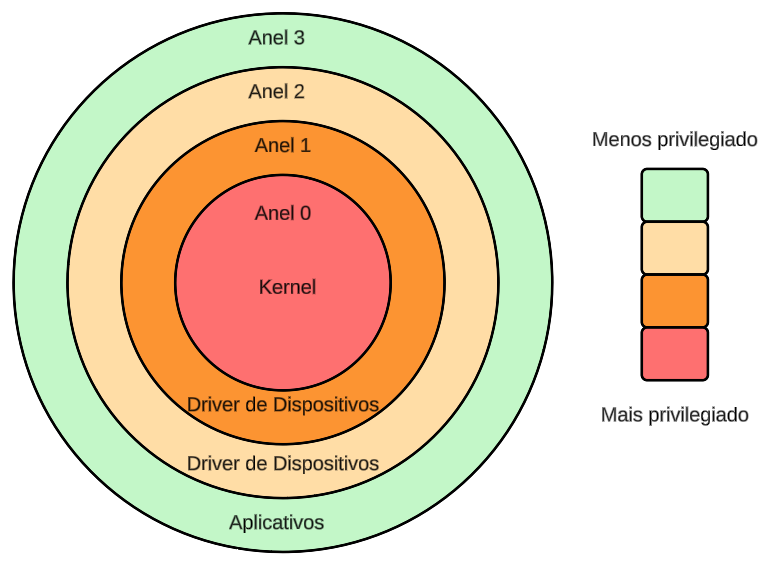
\includegraphics[width=0.7\textwidth]{images/rings_x86.png}
  \label{fig:rings_x86}
\end{figure}

Essa lógica de segurança em formato de anéis ajuda na virtualização e no controle dos \textit{hypervisores}, os quais explicaremos logo em seguida. Os anéis de nível mais baixo, anel 0, têm acesso aos anéis de nível mais alto, anel 3, mas não vice-versa. O SO realiza a segmentação, um método utilizado para definir diferentes regiões da memória com níveis de privilégio distintos. No Linux e na maioria dos sistemas operacionais modernos, o que mais importa é o anel 3 (user mode), menos privilegiado, e o anel 0 (kernel mode), mais privilegiado~\citep{modernOS}. Os demais anéis também são utilizados para armazenar drivers que precisam de mais privilégio que o modo usuário mas menos do que o kernel.

A interação entre o hardware e o sistema operacional na arquitetura x86-64 é fundamental para garantir a segurança e integridade do sistema. Cada anel de privilégio possui um conjunto específico de instruções que pode executar, e o hardware implementa mecanismos que restringem o acesso a essas instruções de acordo com o nível de privilégio. Por exemplo, o código que roda no anel 3, onde estão as aplicações de usuário, não pode executar diretamente instruções privilegiadas que interagem com o hardware, como manipular registros de controle ou acessar diretamente dispositivos de E/S (entrada/saída)~\citep{chirammal2016mastering}. 

Além disso, o hardware utiliza tabelas de descritores de segmentos e tabelas de páginas para garantir que cada anel tenha acesso apenas às porções de memória designadas para seu nível de privilégio. Esses mecanismos previnem, por exemplo, que um código malicioso em anel 3 tente acessar diretamente áreas de memória que pertencem ao kernel ou a outras aplicações. Dessa forma, a combinação de segmentação, gerenciamento de memória e controle de instruções pelo hardware e SO forma uma barreira eficaz contra violações de segurança~\citep{chirammal2016mastering}.



\subsection{\textit{hypervisor} ou VMM}

Ao lidarmos com máquinas virtuais (VMs), é essencial contar com um serviço que gerencie essas instâncias de maneira eficiente, permitindo que possamos iniciar, excluir e replicar nossas máquinas de forma organizada. Esse serviço é desempenhado pelo \textit{hypervisor}, cujo papel é fornecer suporte a múltiplas cópias do hardware físico~\citep{modernOS}. Nos hypervisores modernos, é possível visualizar detalhes de cada VM em execução, como logs, utilização de recursos, tráfego de rede, entre outros aspectos. Além disso, o \textit{hypervisor} é responsável por definir como a VM será construída e como interagirá com o sistema operacional principal~\citep{chirammal2016mastering}.

O \textit{hypervisor} desempenha um papel crucial na tradução de chamadas de sistema (syscalls). Quando uma VM executa uma função crítica, não é viável conceder acesso irrestrito ao hardware, devido a questões de escalabilidade e segurança~\citep{modernOS}. Para resolver esse problema, o \textit{hypervisor} realiza modificações nas chamadas críticas, permitindo que a VM funcione como um sistema operacional principal, conforme ilustrado na Figura \ref{fig:binary_translate} onde temos os serviços separados em aneis com o \textit{hypervisor} no anel 0 e no anel 1 o sistema operacional reescrevendo os binários antes da execução e fazendo a emulação. Dessa forma, o \textit{hypervisor} impede que a VM tenha acesso irrestrito ao hardware. Por exemplo, quando a VM tenta acessar diretamente um recurso específico, como a memória, o \textit{hypervisor} intercepta essa solicitação e a traduz, garantindo a segurança e o controle. Assim, a VM só consegue visualizar o espaço de memória que lhe foi alocado.

\begin{figure}[htbp]
  \centering
  \caption{Tradução de binários em \textit{hypervisores}. A figura ilustra a separação em anéis de proteção, com o \textit{hypervisor} operando no anel 0 e o sistema operacional convidado no anel 1. O \textit{hypervisor} intercepta e reescreve binários críticos antes da execução, realizando a emulação e garantindo a segurança ao evitar o acesso direto ao hardware.}
  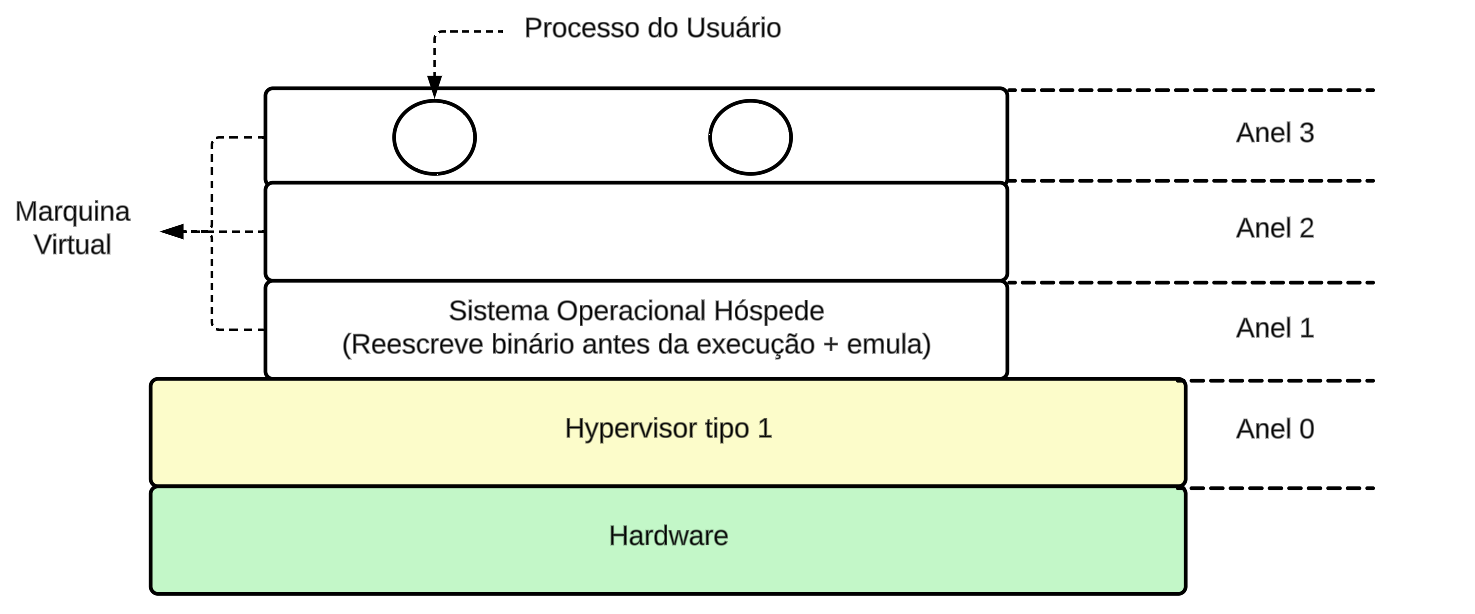
\includegraphics[width=0.7\textwidth]{images/BinaryTranslate.png}
  \caption*{\textit{Fonte:} Adaptado de Modern Operating Systems~\citep{modernOS}.}
  \label{fig:binary_translate}
\end{figure}


As arquiteturas de \textit{hypervisores} também podem variar bastante de um sistema operacional para outro. No caso do Windows, o \textit{hypervisor} mais utilizado é o Hyper-V, que também é a solução adotada pela Azure para a implementação de sua infraestrutura como serviço (IaaS) \href{https://learn.microsoft.com/pt-br/azure/architecture/reference-architectures/n-tier/high-security-iaas}. No entanto, nesta pesquisa, nosso foco será no sistema operacional Linux, devido à sua predominância no mercado de servidores~\citep{OperationSystemMarketVolume} e ao fato de ser open-source~\citep{WhyUseLinux}. Especificamente, abordaremos o \textit{hypervisor KVM (Kernel-based Virtual Machine)}, que é amplamente utilizado nos principais provedores de IaaS, como AWS e Google.


\subsection{\textit{hypervisor} Tipo 1 (Nativo ou Bare Metal)}

A Figura \ref{fig:hypervisor_type01} ilustra o \textit{hypervisor} tipo 1, que é o mais utilizado quando estamos falando de IaaS, o motivo é que ele opera junto ao hardware, as chamadas críticas são feitas diretas no kernel do OS aumentando sua performance~\citep{chirammal2016mastering}, um exemplo notável é o \textit{hypervisor KVM} do Linux. Ele consegue transformar kernel do Linux em um \textit{hypervisor} fazendo com que a VM seja vista como um processo dentro do sistema, como podemos ver na imagem não temos camadas itermediárias para rodar o \textit{hypervisor}, ele roda junto ao \textit{hardware}.


\begin{figure}[h!]
  \centering
  \caption{\textit{Hypervisor} do tipo 1. A imagem ilustra a operação direta com o hardware, onde não há camadas intermediárias entre o \textit{hypervisor} e o \textit{hardware}, aumentando a performance.}
  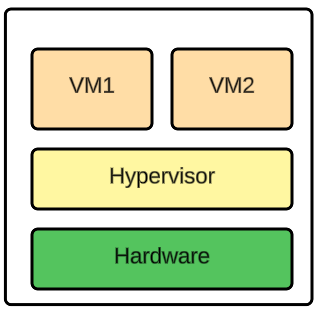
\includegraphics[width=0.4\textwidth]{images/hypervisor_type_1.png}
  \caption*{\textit{Fonte:} Adaptado de~\citep{chirammal2016mastering}.}
  \label{fig:hypervisor_type01}
\end{figure}


Perceba que no bare metal não temos a ideia de um host OS, o hypervsior está direto com o hardware porque roda junto ao kernel.


\subsection*{\textit{hypervisor} Tipo 2 (Hospedeiro)}

O \textit{hypervisor} tipo 2, mostrado na figura \ref{fig:hypervisor_type02}, requer um sistema operacional host principal para funcionar, sendo útil pela facilidade de manuseio e instalação. No entanto, ele não é a melhor opção quando se necessita de alta performance e escalabilidade. Isso se deve, claramente, às camadas adicionais de software que ele introduz. Diferentemente de um \textit{hypervisor} bare metal, o \textit{hypervisor} hospedeiro gera uma sobrecarga maior por operar dentro de um sistema operacional, resultando em chamadas de sistema que são intermediadas pelo \textit{host OS}. Essa configuração cria uma camada de abstração adicional, que pode reduzir a eficiência nas operações críticas.


\begin{figure}[htbp]
  \centering
  \caption{\textit{hypervisor} do tipo 2. A imagem mostra a necessidade de um sistema operacional hospedeiro para o funcionamento do \textit{hypervisor}.}
  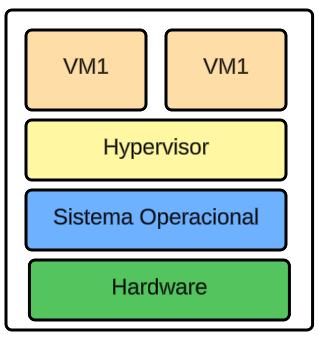
\includegraphics[width=0.4\textwidth]{images/hypervisor_type_2.png}
  \caption*{\textit{Fonte:} Adaptado de \citep{chirammal2016mastering}.}
  \label{fig:hypervisor_type02}
\end{figure}


Neste caso o \textit{hypervisor} e visto de fato como um serviço a parte que está executando no sitema operacional e a VM será vista como um filho desse serviço.


\section{Virtualizações}

Existem três grandes formas de efetuar a virtualização por meio do \textit{hypervisor}, cada uma utilizando características específicas que podem ser aplicadas em diferentes cenários.

\subsection{Virtualização Completa \textit{(Full Virtualization)}}

Neste método, o \textit{hypervisor} emula o hardware para permitir que o sistema operacional convidado (\textit{Guest OS}) opere como se estivesse em uma máquina física independente como monstrado na figura \ref{fig:full_virtualization_rings}. Não há necessidade de modificações no sistema operacional convidado, pois ele não sabe que está sendo virtualizado. Praticamente todas as funções são traduzidas pelo \textit{hypervisor}, evitando chamadas diretas da VM para o kernel do host. O \textit{Guest OS} roda no anel 1, enquanto a máquina virtual (\textit{Virtual Machines Monitor} - VMM) roda no anel 0~\citep{chirammal2016mastering}.

\begin{figure}[htbp]
  \centering
  \caption{Virtualização completa nos anéis de segurança. A figura demonstra o \textit{Guest OS} operando no anel 1 e o VMM no anel 0, com o \textit{hypervisor} realizando a emulação.}
  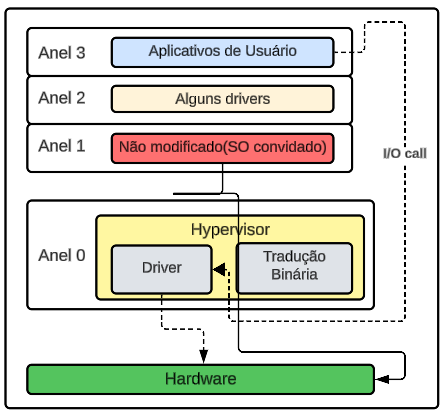
\includegraphics[width=0.6\textwidth]{images/full_virtualization_rings.png}
  \caption*{\textit{Fonte:} Adaptado de~\citep{chirammal2016mastering}.}
  \label{fig:full_virtualization_rings}
\end{figure}


Esse estilo de virtualização utiliza o mecanismo \textit{Trap and Emulate} (Armadilha e Emulação). Quando o \textit{Guest OS} tenta acessar um endereço de memória indevido, o acesso é capturado e emulado pelo \textit{hypervisor}~\citep{chirammal2016mastering}, o que pode gerar uma sobrecarga maior no sistema.

\subsection{Paravirtualização}

Nesse caso, o \textit{Guest OS} é modificado para interagir diretamente com o \textit{hypervisor}, resultando em um desempenho melhor em comparação à virtualização completa. As instruções sensíveis são removidas, e, em vez disso, o sistema operacional realiza chamadas diretas ao \textit{hypervisor} para operações como E/S e mudanças em registros críticos, similar a como programas de aplicação fazem chamadas de sistema em Linux~\citep{modernOS}.

A figura \ref{fig:paravirtualization_rings} mostra como o SO convidado modificado realiza chamadas críticas diretamente para o \textit{hypervisor} por meio de \textit{hypercalls}. Como o SO foi adaptado para trabalhar nesse ambiente, o tratamento de chamadas sensíveis se torna mais eficiente, reduzindo a necessidade de simulação todas as instruções.

\begin{figure}[htbp]
  \centering
  \caption{Paravirtualização nos anéis de segurança. A figura mostra como o sistema operacional convidado modificado realiza chamadas críticas diretamente para o \textit{hypervisor} por meio de hypercalls, tornando o tratamento mais eficiente e reduzindo a necessidade de emulação.}
  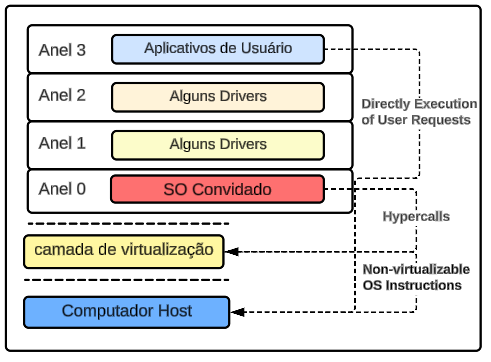
\includegraphics[width=0.6\textwidth]{images/paravirtualization_rings.png}
  \caption*{\textit{Fonte:} Adaptado de~\citep{chirammal2016mastering}.}
  \label{fig:paravirtualization_rings}
\end{figure}

O \textit{Guest OS} opera no anel zero, aproveita as modificações nas chamadas críticas e evitar ações indevidas para reduzir a sobrecarga tornando mais performático que a virtualização completa.

\subsection{Virtualização Assistida por Hardware}

A forma mais eficiente de virtualização é a assistida por hardware, que utiliza recursos nativos do processador, como Intel VT-x ou AMD-V, para executar funções de virtualização diretamente no hardware. Além disso, funções nativas do kernel Linux podem ser utilizadas para otimizar o controle das VMs~\citep{chirammal2016mastering}. Quando uma instrução sensível é executada, o hardware captura a operação e a passa ao \textit{hypervisor} para emulação~\citep{modernOS}.

A figura \ref{fig:hardware_assisted_rings} apresenta uma visão esquemática dos diferentes anéis de privilégio utilizados na virtualização assistida por hardware. Nela, o \textit{Guest OS} opera no anel zero, o mesmo nível de privilégio em que um sistema operacional tradicional funcionaria em uma máquina física, enquanto o \textit{hypervisor} assume um papel central no anel -1, criado especificamente para gerenciar diretamente o acesso ao hardware. Essa estrutura permite que o \textit{hypervisor} intercepte chamadas sensíveis e controle os recursos de forma eficiente, enquanto o sistema convidado e suas aplicações continuam a operar como se tivessem controle completo sobre o hardware subjacente.

\begin{figure}[htbp]
  \centering
  \caption{Virtualização assistida por hardware nos anéis de segurança. A figura mostra o \textit{Guest OS} operando no anel 0 e o \textit{hypervisor} no anel -1, permitindo um gerenciamento eficiente do hardware e reduzindo a necessidade de emulação por software.}
  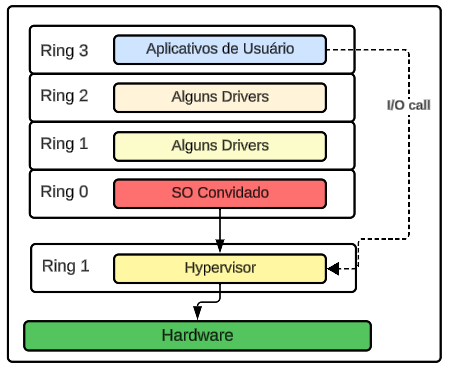
\includegraphics[width=0.6\textwidth]{images/hardware_assisted_rings.png}
  \caption*{\textit{Fonte:} Adaptado de ~\citep{chirammal2016mastering}.}
  \label{fig:hardware_assisted_rings}
\end{figure}

A virtualização assistida por hardware se destaca pela eficiência porquê o processador fica responsável por lidar diretamente com operações sensíveis, eliminando a necessidade de emular essas instruções no software. Essa abordagem reduz a latência associada às traps e minimiza o impacto no desempenho causado pela invalidação de caches e TLBs. O uso de anéis de privilégio dedicados, como o anel -1 para o \textit{hypervisor}, permite que os sistemas convidados operem de forma isolada e com alta performance, enquanto o \textit{hypervisor} gerencia as interações críticas com o hardware de maneira otimizada~\citep{chirammal2016mastering}.

\subsection{Considerações sobre os tipos de virtualização}

Não são apenas as funções críticas que são traduzidas pelo \textit{hypervisor}. Utilizando a tecnologia VT (Virtualization Technology), o hardware gera uma grande quantidade de interrupções, conhecidas como traps. Essas traps podem prejudicar significativamente o desempenho do sistema, pois invalidam o cache da CPU e os TLBs \textit{(Translation Lookaside Buffers)}, que são ewssenciais para o rápido acesso à memória. Quando o cache e os TLBs são invalidados, a CPU precisa recarregar essas informações, o que aumenta a latência e reduz a eficiência geral. Para mitigar esses efeitos negativos, o \textit{hypervisor} captura e traduz algumas funções não críticas. Isso é feito para reduzir a frequência das traps e, consequentemente, diminuir o impacto sobre o desempenho. Ao gerenciar melhor quais funções precisam ser interceptadas e traduzidas, o \textit{hypervisor} pode manter um equilíbrio entre a funcionalidade e a eficiência do sistema~\citep{modernOS}.

Lembrando que essas 3 são formas gerais de virtualização, como serão feitas as traduções binárias das funções críticas a emulação entre outros detalhes vai depender do \textit{hypervisor} que está sendo utilizado. Nenhuma instrução sensível emitida pelo sistema operacional hóspede jamais é executada diretamente pelo verdadeiro hardware. Elas são transformadas em chamadas pelo \textit{hypervisor}, que então as emula~\citep{modernOS}.

Como estamos falando que computação em nuvem nosso foco vai ser o \textit{hypervisor} do tipo 1 e com a virtualização assistida pelo hardware utilizado pelo OpenStack, o mótivo dessa escolha é pelos detalhes que falamos a cima, precisamos do máximo de performace possível e alta escalabilidade, o OpenStack aceita vários tipos de \textit{hypervisors} mas por padrão é utilizado o QEMU/KVM~\citep{DocumentacaoOpenstack}.


\section{Importância das Tecnologias de Virtualização para VMs}

Tecnologias como o KVM \textit{(Kernel-based Virtual Machine)} e ferramentas como o Libvirt proporcionam uma base robusta para a criação, gerenciamento e escalabilidade de VMs, enquanto a virtualização assistida por hardware e técnicas de alocação de recursos (CPU, memória e rede) garantem que as VMs operem com alto desempenho. Estas tecnologias são indispensáveis para qualquer infraestrutura moderna que dependa de VMs para suportar suas operações e demandas em ambientes complexos e de larga escala.

\subsection{Libvirt - API e VMs}
O \textit{libvirt} é amplamente utilizado em diversos serviços que gerenciam máquinas virtuais (VMs), sendo uma biblioteca essencial para simplificar a criação e administração dessas VMs. Ele oferece uma interface unificada e de fácil utilização para diferentes tecnologias de virtualização, c1omo o QEMU, que, por sua vez, utiliza o KVM para aproveitar a aceleração por hardware. Além disso, o \textit{OpenStack}, por meio do serviço \textit{NOVA}, utiliza o \textit{libvirt} para a orquestração de VMs ~\citep{DocumentacaoOpenstack}; \href{https://docs.openstack.org/kolla-ansible/latest/reference/compute/libvirt-guide.html}{\textit{libvirt guide}}.

Um exemplo de criação de uma máquina virtual utilizando o \textit{libvirt} com QEMU-KVM pode ser feito através do comando \texttt{virt-install} diretamente no terminal, passando os parâmetros de configuração desejados. Esses parâmetros são convertidos em um arquivo XML que descreve as especificações da VM. Esse arquivo, geralmente localizado em \texttt{/etc/libvirt/qemu}, pode ser editado manualmente conforme necessário. O QEMU, em conjunto com o KVM, utiliza essas informações para configurar e iniciar a máquina virtual de maneira otimizada. Por padrão, se o KVM estiver disponível no sistema, ele será utilizado para melhorar o desempenho da VM.

O \textit{libvirt} é, na verdade, um conjunto de APIs chamado ``Virtualization API'', que permite o gerenciamento padronizado de várias plataformas de virtualização, como KVM, QEMU, Xen, VMware, Hyper-V, e LXC. Essas APIs fornecem uma camada de abstração, permitindo que diferentes \textit{hypervisors} sejam controlados de maneira uniforme e consistente~\citep{chirammal2016mastering}. Isso torna o \textit{libvirt} uma ferramenta central em ambientes de virtualização complexos e escaláveis.

Como mostrado da figura \ref*{fig:libvirt_interface}, ele utiliza dos \textit{driver} de cada \textit{hypervisor}, os \textit{drivers} são descobertos durante o processo de conexão com a API. Cada \textit{driver} tem uma API de registro que carrega as referências de função específicas do \textit{driver} para as APIs libvirt chamarem, assim como os respectivos protocolos utilizados por essas APIs. A arquitetura do \textit{driver} também é usada para dar suporte a outros componentes de virtualização, como armazenamento, pools de armazenamento, dispositivo host, rede, interfaces de rede e filtros de rede~\citep{LibvirtDocumentation}. Um exemplo simples de XML configurado para 1 vCPU utilizando o KVM e o QEMU, armazenando a imagem no arquivo do tipo QCOW2 pode ser visto em Código \ref{code:example_kvm_qemu}.


\begin{figure}[htbp]
  \centering
  \caption{Interface para drivers do \textit{libvirt}. A figura ilustra como o \textit{libvirt} se conecta a diferentes hypervisores por meio de drivers específicos, permitindo o gerenciamento padronizado de componentes de virtualização, como rede, armazenamento e dispositivos.}
  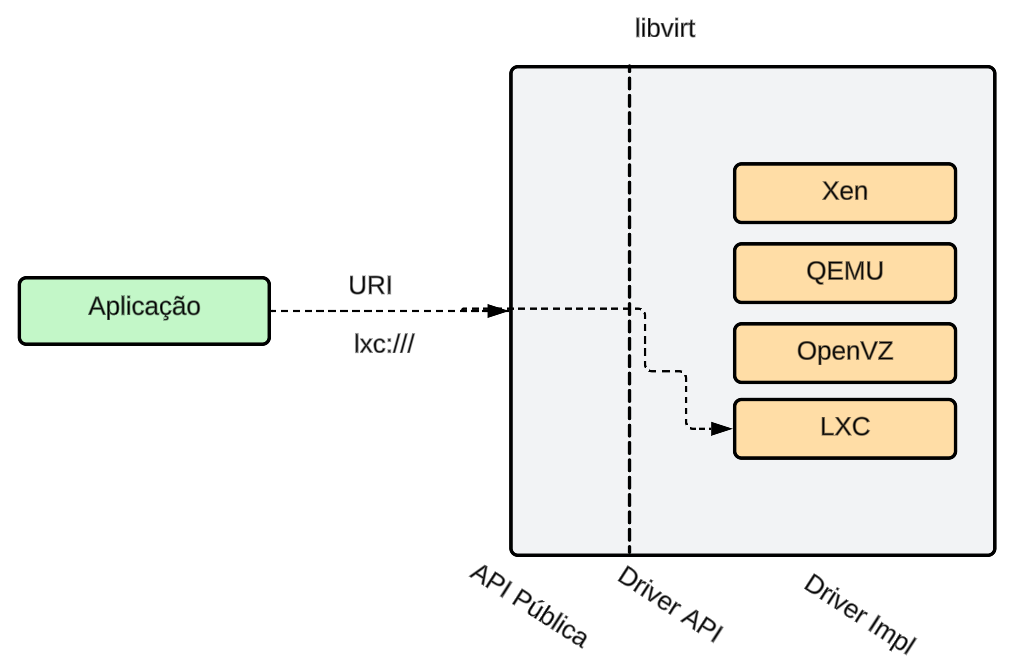
\includegraphics[width=0.7\textwidth]{images/libvirt_interface.png}
  \caption*{\textit{Fonte:} Adaptado de~\citep{LibvirtDocumentation}.}
  \label{fig:libvirt_interface}
\end{figure}

\begin{listing}[h!]
  \noindent\fcolorbox{black}{gray!10}{%
  \parbox{\textwidth}{%
    \inputminted[]{html}{files/example.xml}
  }%
}  
\caption{Exemplo de configuração em XML para uma VM utilizando KVM e QEMU. O arquivo define as especificações da máquina virtual, incluindo uma vCPU, memória, tipo de armazenamento em formato QCOW2, e outras configurações essenciais para a inicialização e operação da VM.}
\label{code:example_kvm_qemu}
\end{listing}


O código \ref{code:example_kvm_qemu} contém as informações necessárias para configurar a VM, incluindo a memória, quantidade de vCPUs, imagem de carregamento, tipo de arquivo, entre outras configurações.

Naturalmente, para salvar o storage das VMs, utilizamos o arquivo QCOW2 \textit{(QEMU Copy On Write version 2)}. Ele possui diversas funcionalidades que ajudam no manuseio das imagens e na escalabilidade. Sua estrutura foi desenhada pelo QEMU pensando no manuseio de VMs, por isso inclui recursos como snapshots, compressão, encriptação e redimensionamento dinâmico.


\subsection{KVM - \textit{Kernel-based Virtual Machine}}

O \textit{\textbf{Kernel-based Virtual Machine (KVM)}}, como comentado acima, interage com o kernel para formar um poderoso hipervisor tipo 1 para sistemas operacionais baseados em Linux, amplamente utilizado em serviços de nuvem. Ele permite a orquestração de VMs com funções integradas diretamente ao kernel e oferece virtualização assistida por hardware.

O KVM não funciona como um serviço independente, ele precisa estar integrado ao kernel do Linux e depende da assistência de hardware para virtualização (VT-X), utilizando módulos específicos como os encontrados em \textit{kvm-intel.ko}. Além disso, o KVM também precisa do \textbf{QEMU}, que fornece os binários necessários para a construção e gerenciamento das VMs. Juntos, KVM e QEMU formam um hipervisor robusto, capaz de controlar várias VMs, oferecendo uma solução de virtualização escalável e eficiente~\citep{chirammal2016mastering}.

De forma geral, o módulo de kernel do KVM é responsável por diversas funções críticas~\citep{chirammal2016mastering}:

\begin{itemize}
    \item \textbf{Gestão de CPUs Virtuais (vCPUs)}: O KVM gerencia vCPUs, que são \textit{threads} POSIX criadas para cada VM, permitindo a execução de instruções diretamente no kernel do sistema operacional.
  
    \item \textbf{Gerenciamento de Memória}: Utiliza \textit{EPT (Extended Page Tables)} ou \textit{NPT (Nested Page Tables)} para gerenciar a memória alocada para cada VM, assegurando o mapeamento eficiente entre a memória virtual da VM e a memória física do host.

    \item \textbf{Manuseio de \textit{Threads} de I/O}: Facilita a comunicação entre dispositivos virtuais e o hardware físico, interceptando e encaminhando operações de I/O.

    \item \textbf{Interrupções e Exceções}: Lida com interrupções e exceções geradas por chamadas críticas, utilizando virtualização assistida por hardware para emular respostas apropriadas.

    \item \textbf{Controle e Monitoramento}: Expondo uma interface por meio de \textit{ioctls}, o KVM permite a configuração, controle e monitoramento das VMs.

    \item \textbf{Segurança e Isolamento}: Garante a segurança e o isolamento das VMs, controlando o acesso a cada espaço de memória e evitando interferências entre as VMs.
\end{itemize}

Na figura \ref{fig:qemu_kvm_architecture}, é ilustrada a arquitetura do hipervisor \textit{QEMU/KVM}, mostrando como o QEMU e o KVM interagem para emular uma virtualização, gerenciar vCPUs e realizar transições entre os modos do host e do convidado. Na seção superior, o modelo de máquina virtual exibe componentes como o subsistema de E/S e os threads da CPU responsáveis pela execução das instruções da VM. Já a seção inferior destaca o papel do KVM, que utiliza APIs específicas e tabelas de páginas estendidas (\textit{EPT}) para gerenciar memória e executar VMs em modo convidado, enquanto monitora eventos de saída (\textit{VM Exit}) e lida com interrupções, entradas/saídas e violações de página. Essa integração entre QEMU e KVM resulta em uma infraestrutura robusta para virtualização assistida por hardware, assegurando desempenho e isolamento entre as VMs.

\begin{figure}[htbp]
  \centering
  \caption{Arquitetura do \textit{hypervisor} \textit{QEMU/KVM}. A figura ilustra a interação entre o QEMU e o KVM, mostrando o gerenciamento de vCPUs, E/S e memória, além das transições entre o modo do host e do convidado para virtualização assistida por hardware.}
  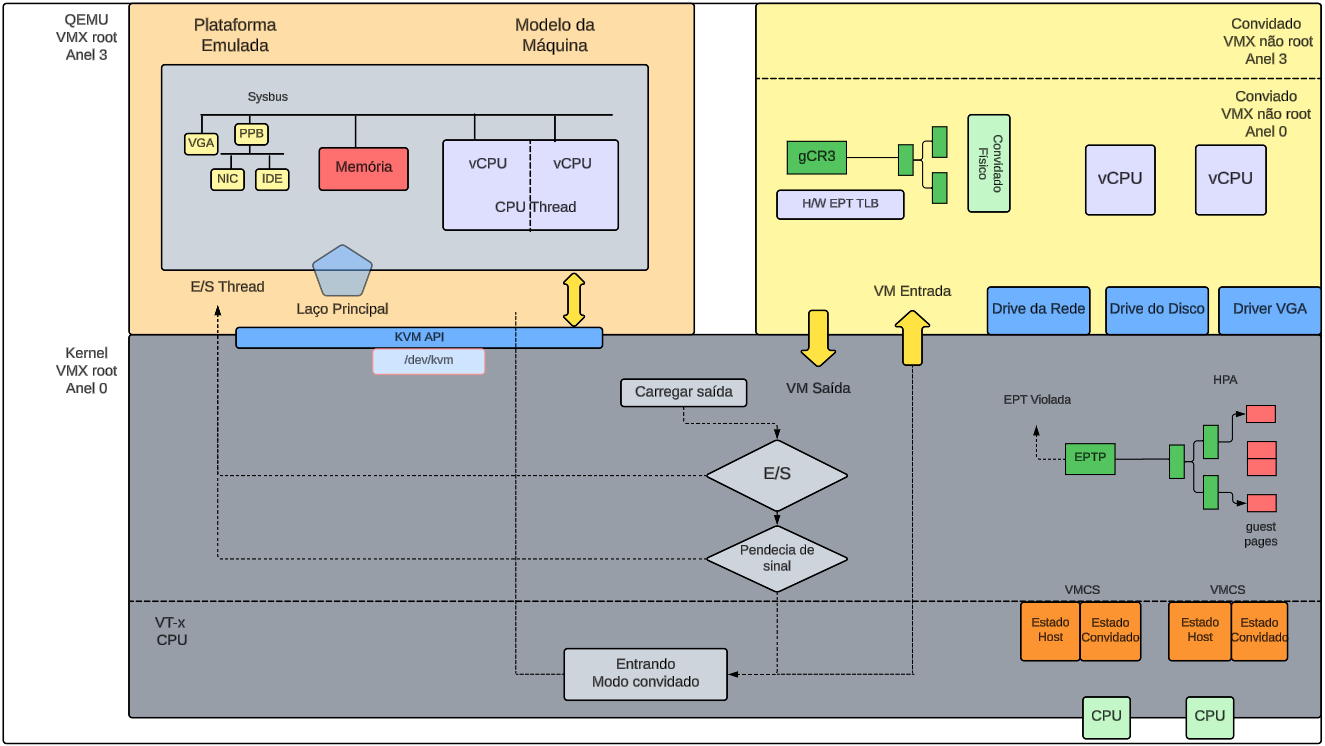
\includegraphics[width=0.9\textwidth]{images/qemu_kvm_architecture.png}
  \caption*{\textit{Fonte:} Adaptado de \url{https://wiki.qemu.org/Documentation/Architecture}.}
  \label{fig:qemu_kvm_architecture}
\end{figure}


\subsection{VMX para o KVM}

O \textit{\textbf{VMX}} é substancial para o \textit{\textbf{KVM}}, que utiliza as funções \textit{VM*} disponibilizadas pela tecnologia de hardware assistido. Essas funções são usadas para o controle da VM e são disponibilizadas pelo \textbf{KVM} para que outros serviços de mais alto nível possam acessá-las através dos \textit{ioctls} (\textit{input/output control})~\citep{wiki:Ioctl}, que ficam em \textit{/dev/kvm}. Alguns exemplos de funções disponibilizadas pelo hardware são:

\begin{itemize}
  \item \textbf{VMREAD}: Lê o conteúdo de um campo de controle específico da VM.
  \item \textbf{VMWRITE}: Escreve um valor em um campo de controle específico da VM.
  \item \textbf{VMCLEAR}: Limpa a estrutura da VM.
  \item \textbf{VMPTRLD}: Carrega o ponteiro para a estrutura da VM.
  \item \textbf{VMLAUNCH}: Inicia a execução da VM.
  \item \textbf{VMRESUME}: Retoma a execução da VM após uma interrupção.
\end{itemize}

Essas funções interagem com o KVM através de chamadas ao \textit{ioctl}. O \textit{\textbf{KVM}} fornece uma interface que os usuários podem utilizar para configurar e controlar VMs, e essa interface faz uso das funções \textit{VMX} para manipular diretamente o estado e a execução das VMs no nível do hardware~\citep{zabaljauregui2008hardware}. Existem diversas outras chamadas que são utilizadas.

Essa relação é de extrema importância para o \textit{\textbf{QEMU-KVM}}, pois o \textit{\textbf{QEMU}} utiliza as chamadas \textit{ioctls} disponibilizadas na interface do KVM para se comunicar com o hardware de maneira mais eficiente.

\subsection{Alocação de CPU}

Como comentado, uma vCPU, que é a CPU da VM, é implementada como uma \textit{thread} POSIX. Isso significa que ela funciona como uma conexão ao CPU físico, com funções que ajudam a controlá-la. Essas \textit{threads} são semelhantes a qualquer outra \textit{thread} no sistema operacional \textit{host} em termos de execução~\citep{chirammal2016mastering}.

A forma como cada vCPU será processada depende de como o escalonador do Linux irá tratá-la. O escalonador do Linux gerencia a alocação de tempo de CPU para todas as \textit{threads}, incluindo aquelas que representam vCPUs. Em geral, podemos esperar uma média de 2 \textit{threads} vCPU para cada núcleo físico da CPU, embora isso possa variar dependendo da aplicação e do hardware utilizado~\citep{TechTargetvCPU}.

\subsection{Alocação de Memória}

A alocação de memória é uma parte crítica no processo de criação e gerenciamento de máquinas virtuais (VMs). Cada VM precisa de sua própria área de memória para operar, e o gerenciamento dessa memória é essencial para garantir que o sistema \textit{host} possa suportar múltiplas VMs simultaneamente sem sobrecarregar os recursos disponíveis. De forma geral, cada VM possui suas próprias tabelas de páginas que mapeiam endereços de memória virtual para endereços de memória física~\citep{modernOS}.

No contexto de sistemas como \textit{QEMU/KVM}, por exemplo, a alocação de memória envolve a leitura de um arquivo de configuração (como um XML) que especifica a quantidade de memória necessária para a VM. A memória especificada é então reservada no espaço de endereço do processo, e o \textit{hypervisor} (textit{KVM}, neste caso) é responsável por criar as páginas de memória necessárias para traduzir os endereços de memória virtual da VM para a memória física do \textit{host}~\citep{chirammal2016mastering}.

\subsection{Virtualização na Placa de Rede}

Para que todas as VMs de uma máquina tenham acesso a uma rede, precisamos de três componentes principais: \textit{Hypervisor}, NICs virtuais (\textit{Network Interface Controller}) e os Switches Virtuais. Cada VM possui sua própria vNIC com endereço MAC (\textit{Media Access Control}) e IP (\textit{Internet Protocol}) próprios. 

O \textit{switch} virtual (vSwitch) é um componente essencial que permite a comunicação entre as vNICs e a NIC real. Ele funciona como um \textit{switch} normal, encaminhando pacotes entre as vNICs e a rede física, permitindo que todas consigam se comunicar.

O \textbf{SR-IOV} (\textit{Single Root I/O Virtualization}) é outra tecnologia importante para a virtualização. Ele permite que uma única NIC física apresente múltiplas interfaces lógicas, como mostrado na figura \ref{fig:single_root_IO_virtualization}. Cada interface lógica é chamada de VF (\textit{Virtual Function}). Naturalmente, cada VF é atribuída a uma VM, permitindo acesso direto ao hardware da NIC, melhorando a performance~\citep{dong2012high}, enquanto a PF (\textit{Physical Function}) compartilha recursos com as VFs.

\begin{figure}[htbp]
  \centering
  \caption{Arquitetura SR-IOV. A figura ilustra como uma única NIC física pode apresentar múltiplas interfaces lógicas (\textit{Virtual Functions} - VFs), permitindo que cada VM tenha acesso direto ao hardware, enquanto a \textit{Physical Function} (PF) gerencia os recursos compartilhados.}
  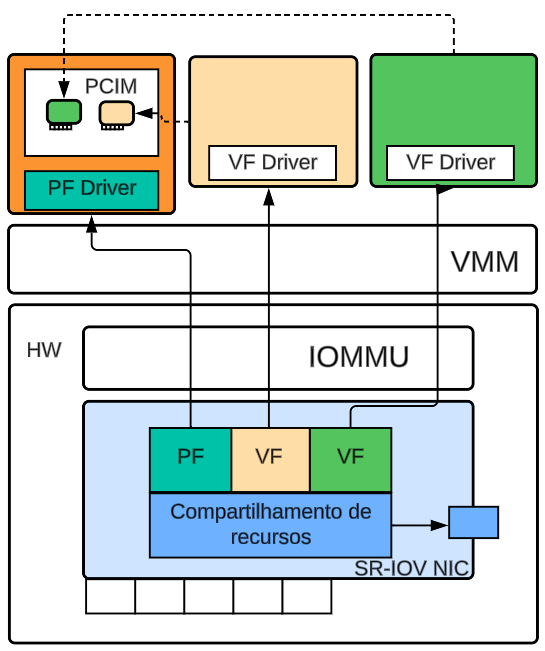
\includegraphics[width=0.5\textwidth]{images/single_root_IO_virtualization.png}
  \caption*{\textit{Fonte:} Adaptado de~\citep{dong2012high}.}
  \label{fig:single_root_IO_virtualization}
\end{figure}


Junto a todas essas tecnologias, utilizamos também algoritmos para efetuar o balanceamento de carga, como \textit{Round-Robin}, \textit{Least Connections} e \textit{Weighted Fair Queuing}, usados para distribuir o tráfego de maneira eficiente entre várias VMs~\citep{dong2012high}.


\section{Containers}

Container é uma forma leve de virtualização que permite isolar processos e seus recursos em um ambiente controlado e consistente. Os containers compartilham o mesmo \textit{kernel} do sistema operacional, mas são isolados uns dos outros e do sistema \textit{host}, proporcionando uma maneira eficiente de executar aplicações com suas dependências em um ambiente previsível.

O \textbf{LXC} (\textit{Linux Containers}) foi a primeira grande implementação dos containers como conhecemos hoje em dia~\citep{HistoryOfCloudByIBM}, um serviço isolado executando com uma certa limitação de hardware e de fácil criação. Esse novo sistema serviu de inspiração para o desenvolvimento de grandes serviços usados na indústria hoje em dia, como o \textbf{Docker}.

De forma geral, os containers são criados utilizando tecnologias existentes dentro do sistema operacional. No caso dos sistemas baseados em \textit{Unix}, utilizam-se as tecnologias de \textit{namespaces} e \textit{cgroups}. Iremos destacar melhor como cada uma dessas tecnologias funciona, mas, basicamente, utilizamos essas tecnologias para fazer a limitação de recursos e separação de acesso lógico.

Quando comparamos a infraestrutura necessária para executar uma VM ou um container, percebemos que, de fato, ocorre uma diminuição de \textit{overhead}. A VM precisa de emulação de hardware, enquanto o container é apenas software~\citep{OCIContainer}, como mostrado na figura \ref{fig:vm_x_container}. No caso dos containers, eles também compartilham o mesmo \textit{host kernel}, o que gera maior facilidade na hora de escalar a quantidade de containers.


\begin{figure}[htbp]
  \centering
  \caption{Comparação de arquitetura entre containers e VMs. A figura mostra como os containers compartilham o \textit{kernel} do host, enquanto as VMs utilizam um \textit{hypervisor} e requerem emulação de hardware, resultando em maior \textit{overhead} para VMs.}
  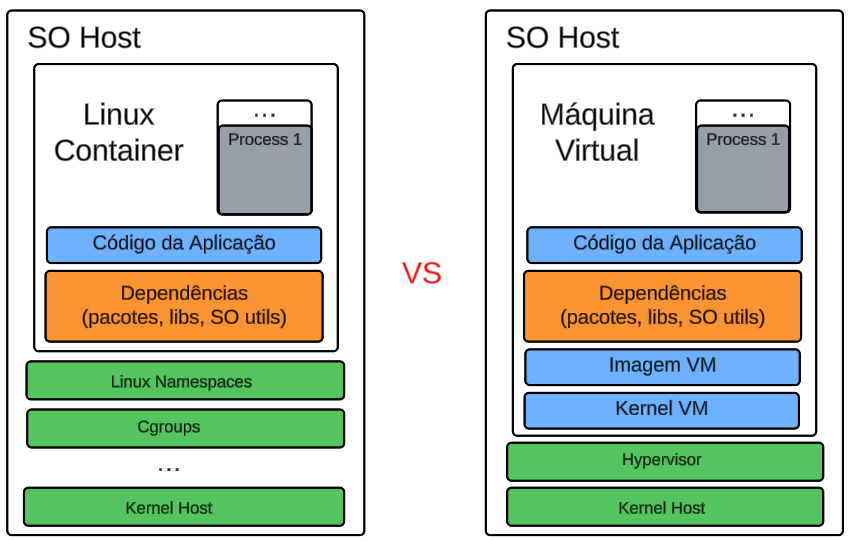
\includegraphics[width=0.7\textwidth]{images/vm_x_container_2.png}
  \caption*{\textit{Fonte:} Adaptado de~\citep{OCIContainer}.}
  \label{fig:vm_x_container}
\end{figure}


\subsection{Namespaces}

Atualmente, o Linux implementa sete tipos diferentes de \textit{namespaces}. O propósito de cada \textit{namespace} é encapsular um recurso de sistema global específico em uma abstração que faz parecer aos processos dentro do \textit{namespace} que eles têm sua própria instância isolada do recurso global. Um dos objetivos gerais dos \textit{namespaces} é dar suporte à implementação de containers, uma ferramenta para virtualização leve que fornece a um grupo de processos a ilusão de que eles são os únicos processos no sistema~\citep{LWNNamespaces}.

Existem \textit{namespaces} essenciais no Linux, cada um com uma tarefa importante no sistema operacional para garantir segurança e isolamento:

\begin{itemize}
  \item \textbf{PID (Identificador de Processo):} Isola os IDs de processos. Dessa forma, processos dentro do \textit{namespace} PID não podem ver processos de fora dele. Isso significa que processos com \textit{namespaces} diferentes podem ter o mesmo PID, porém não têm visibilidade ou interferência uns com os outros. Funciona como um serviço hierárquico: o processo pai tem acesso ao filho, mas isso também pode ser alterado, isolando completamente o processo filho.
  
  \item \textbf{NET (Rede):} Isola interfaces de rede, roteadores, tabelas de roteamento, \textit{firewalls} e \textit{sockets} de rede, permitindo um isolamento completo da rede. Isso significa que cada \textit{namespace} de rede pode ter suas próprias interfaces de rede, rotas, regras de \textit{firewall}, etc., sem interferir nos \textit{namespaces} de rede de outros processos. É frequentemente usado para criar ambientes de rede virtualizados, como containers com suas próprias pilhas de rede.
  
  \item \textbf{MNT (Montagem de Sistemas de Arquivos):} Isola a árvore de sistemas de arquivos montados. Dessa forma, os processos dentro de um \textit{namespace} de montagem têm uma visão diferente dos sistemas de arquivos montados em comparação aos processos fora desse \textit{namespace}. Isso permite ter diferentes sistemas de arquivos ou pontos de montagem visíveis para diferentes processos. Por exemplo, pode-se montar um diretório somente leitura dentro de um container sem afetar o resto do sistema.
  
  \item \textbf{UTS (Identificação do Sistema):} Isola o nome do \textit{host} e o domínio do sistema. Isso permite que cada \textit{namespace} tenha seu próprio nome de \textit{host} e domínio, possibilitando a criação de ambientes isolados que podem parecer sistemas diferentes para os processos dentro deles. É útil para ambientes de teste e desenvolvimento onde diferentes configurações de nome de \textit{host} são necessárias.
  
  \item \textbf{IPC (Comunicação entre Processos):} Isola recursos de IPC, como filas de mensagens, semáforos e memória compartilhada. Isso garante que os processos dentro de um \textit{namespace} de IPC não possam acessar os recursos de IPC fora dele. Esse isolamento é essencial para containers e outros ambientes de virtualização, onde os recursos de IPC precisam ser isolados para garantir a segurança e a estabilidade.
  
  \item \textbf{USER (Identificação do Usuário):} Isola os IDs de usuário e grupos. Isso permite que processos dentro de um \textit{namespace} de usuário tenham uma visão diferente dos IDs de usuário e grupos comparados aos processos fora do \textit{namespace}. É particularmente útil para permitir que processos dentro de containers rodem como \textit{root} dentro do container, mas como um usuário não privilegiado no sistema \textit{host}, aumentando a segurança.
  
  \item \textbf{CGROUP (Grupos de Controle):} Isola a hierarquia de \textit{cgroups}, usados para limitar e isolar o uso de recursos como CPU, memória, disco e rede. Cada \textit{namespace} de \textit{cgroup} pode ter suas próprias regras e limitações, permitindo a alocação e gerenciamento de recursos de forma eficiente e segura. É uma ferramenta essencial para a gestão de recursos em ambientes de containers e virtualização, garantindo que um container não possa monopolizar os recursos do sistema.
\end{itemize}

\subsection{Cgroups}

Os \textit{cgroups}, como mencionado anteriormente, são essenciais para o gerenciamento de recursos da máquina. Eles permitem definir quanto cada processo pode utilizar, complementando o isolamento oferecido pelos \textit{namespaces}. Enquanto os \textit{namespaces} oferecem isolamento lógico, os \textit{cgroups} garantem o isolamento de recursos. Na prática, containers como Docker e LXC possuem funcionalidades adicionais, mas a base deles é o isolamento lógico e de recursos.

Podemos separar diferentes recursos existentes na máquina utilizando o PID do processo. Sempre que um novo processo é iniciado, o sistema operacional atribui um PID, essencial para a identificação no contexto apropriado \href{https://docs.kernel.org/admin-guide/cgroup-v1/cgroups.html}. Existe um diretório padrão para separar os \textit{cgroups}: \texttt{/sys/fs/cgroup/resource}, onde \texttt{resource} representa o recurso a ser isolado.

Para criar um \textit{cgroup} específico, utilizamos o diretório padrão e adicionamos uma nova pasta com o nome do \textit{cgroup}, por exemplo: \texttt{/sys/fs/cgroup/newgroup/resource}. Dentro desta pasta, configuramos como queremos limitar os recursos. Após essa configuração, basta mover o PID para dentro desse novo \textit{cgroup} na pasta \texttt{/tasks}. Nos novos sistemas operacionais baseados em Linux, é utilizado o \textit{cgroup v2}, que altera um pouco a organização dos diretórios; por exemplo, o PID deve ser movido para \texttt{/newgroup/cgroup.procs}. O Código \ref{code:debian_docker} mostra um exemplo de como poderíamos baixar o OS Debian simples apenas com os arquivos necessários para executar o sistema e isolá-lo.


\begin{listing}[h!]
  \noindent\fcolorbox{black}{gray!10}{%
  \parbox{\textwidth}{%
  \inputminted[]{sh}{files/container.sh}
  }%
}  
\caption{Exemplo de script para baixar uma versão mínima do sistema operacional Debian, configurá-lo de forma isolada utilizando \textit{cgroups} e \textit{namespaces}, e executar processos dentro desse ambiente isolado, simulando um container.}
\label{code:debian_docker}
\end{listing}


Após a criação feita no Código \ref{code:debian_docker}, você já pode executar o serviço isolado como um container. Os containers executados por LXC ou Docker possuem diversas outras \textit{features} que ajudam em uma boa integração para microserviços e automatização de \textit{deploy}, isso é apenas um exemplo.

\subsection{Docker}

O \textbf{Docker} é uma plataforma amplamente utilizada para criar, implantar e gerenciar containers, especialmente em contextos de microserviços e escalabilidade horizontal. Ele facilita a criação de ambientes isolados e consistentes para a execução de aplicativos, utilizando a tecnologia de containers junto com diversas outras funcionalidades~\citep{DockerDocumentation}. O Docker foi desenvolvido com base na tecnologia \textbf{Linux Containers (LXC)}.

Uma das principais inovações do Docker foi a implementação do conceito de imagens dentro dos containers, o que simplificou a cópia e reconstrução de ambientes. Imagens de containers são configurações pré-definidas que podem ser utilizadas para criar ambientes de execução idênticos em qualquer lugar~\citep{DockerDocumentation}. Quando uma imagem é copiada e executada, o Docker constrói um ambiente isolado que replica exatamente a configuração daquela imagem. Essa funcionalidade é extremamente útil para desenvolvedores que precisam garantir a replicação precisa de ambientes de desenvolvimento, teste ou produção.

\subsection{Linux Containers - LXC}  
O \textbf{Linux Containers (LXC)} é uma tecnologia de virtualização a nível de sistema operacional que permite a criação de múltiplas instâncias isoladas de ambientes de usuários em um único \textit{host} Linux. Enquanto o Docker popularizou o conceito de containers, o LXC é uma solução mais antiga que oferece uma abordagem semelhante, mas com algumas diferenças em termos de implementação e casos de uso~\citep{WhatIsDocker}.

O LXC funciona utilizando \textit{namespaces} do \textit{kernel} Linux, que fornecem isolamento para processos, além de \textit{cgroups}, que gerenciam a limitação de recursos como CPU, memória e I/O. Isso permite que cada container LXC tenha seu próprio sistema de arquivos, rede, processos e até mesmo dispositivos. Diferente do Docker, que é mais orientado a aplicações, o LXC permite a criação de containers que podem funcionar como sistemas operacionais completos, tornando-se uma solução interessante para ambientes que exigem maior flexibilidade e controle sobre o sistema~\citep{LinuxContainers}.

Em termos de utilização, o LXC é frequentemente gerenciado por ferramentas como o \texttt{lxd}, que fornece uma interface mais amigável e funcionalidades avançadas para administrar containers em larga escala, incluindo suporte a redes complexas, armazenamento em disco e operações de migração ao vivo.

O LXC é extremamente útil para virtualização, mas não oferece uma experiência tão boa para os desenvolvedores. A tecnologia Docker oferece mais do que a habilidade de executar containers: ela também facilita o processo de criação e construção de containers, o envio e o controle de versão de imagens, entre outros~\citep{WhatIsDocker}.


% START OPENSTACK
\section{Introdução ao OpenStack}

O OpenStack é uma plataforma de código aberto composta por uma série de softwares projetados para gerenciar infraestruturas virtualizadas. Desenvolvido com o apoio de uma ampla comunidade de colaboradores, que inclui grandes empresas de tecnologia como VMWare, IBM, Cisco, Red Hat, Canonical, entre outras~\citep{OpenStackIndtroductionUFRJ}, o OpenStack se destaca por ser um projeto \textit{open-source} altamente colaborativo.

Iniciado em 2010 pela Rackspace e NASA, o OpenStack tinha como objetivo criar uma plataforma de computação em nuvem de código aberto que fosse fácil de usar e implementar, além de interoperável entre diferentes implementações e adaptável a diversas escalas~\citep{DocumentacaoOpenstack}

Funcionando como um sistema operacional em nuvem, o OpenStack gerencia grandes conjuntos de recursos de computação, armazenamento e rede em um datacenter~\citep{OpenStackSoftware}. Além de sua função principal como Infraestrutura como Serviço (IaaS), o OpenStack incorpora componentes adicionais que proporcionam orquestração, gerenciamento de falhas e serviços, expandindo suas capacidades para atender às necessidades complexas de ambientes de nuvem.

\section{Arquitetura Geral}

A arquitetura do OpenStack é composta por uma coleção de serviços modulares interconectados, que em conjunto possibilitam o gerenciamento e a automação de recursos de computação, rede e armazenamento. Essa modularidade permite que os administradores personalizem a solução de acordo com as demandas específicas de seus ambientes, integrando apenas os componentes necessários.

Essa flexibilidade faz do OpenStack uma solução escalável, adequada tanto para pequenas nuvens privadas quanto para grandes data centers públicos. A Figura \ref{fig:map_openstack} ilustra como os diferentes componentes do OpenStack se integram para formar uma solução completa de infraestrutura de nuvem.

\subsection{Modelo de Serviço}
O OpenStack segue, como comentado acima, o modelo de IaaS, onde recursos de computação, armazenamento e redes são disponibilizados aos usuários sob demanda. Esses recursos são gerenciados por meio de APIs \textit{(Application Programming Interfaces)}, permitindo que os usuários criem, configurem e administrem sua infraestrutura de maneira programática.

Esse modelo de serviço oferece flexibilidade significativa, permitindo que os recursos sejam provisionados e escalados conforme necessário, sem a necessidade de intervenção manual. O OpenStack automatiza muitas das tarefas tradicionais de gerenciamento de infraestrutura, como alocação de recursos, monitoramento de desempenho e aplicação de políticas de segurança, facilitando a administração e garantindo alta disponibilidade e eficiência dos recursos.

Na Figura \ref{fig:map_openstack}, é possível observar os principais componentes oferecidos pelo OpenStack e suas respectivas áreas de interação. Por exemplo, Neutron, Octavia e Designate atuam na área de \textit{Network}, enquanto Nova e Zun estão relacionados à \textit{Compute}, entre outros.


\begin{figure}[htbp]
    \centering
    \caption{Mapa dos componentes do OpenStack. A figura apresenta os principais serviços do OpenStack, destacando suas áreas de atuação, como \textit{Compute}, \textit{Network} e \textit{Storage}, e ilustrando como esses serviços interagem para fornecer uma solução de nuvem completa.}
    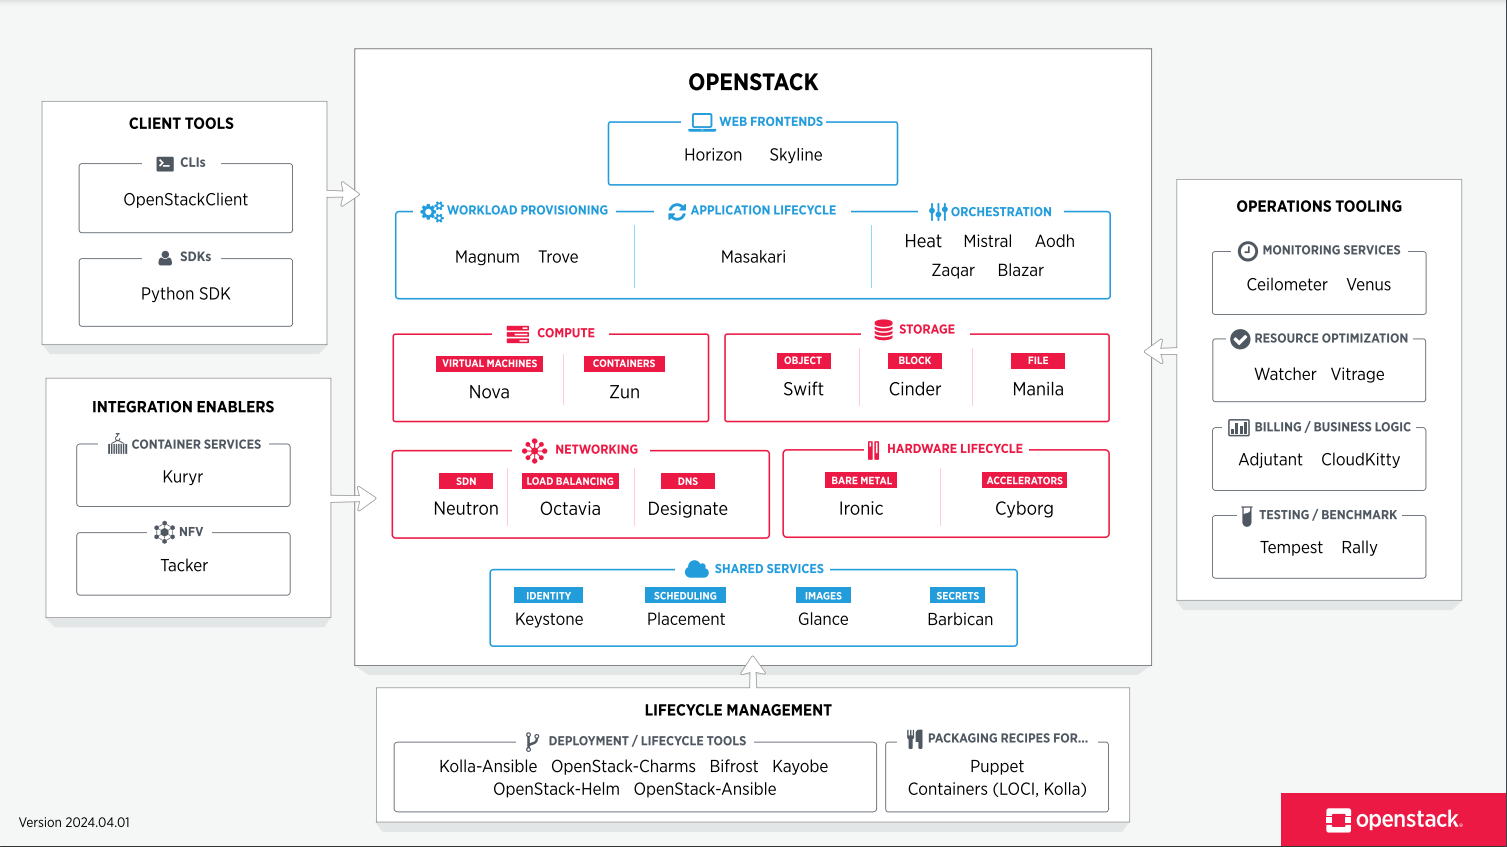
\includegraphics[width=1.0\textwidth]{images/map_openstack.png}
    \caption*{\textit{Fonte:} \url{https://www.openstack.org/software}.}
    \label{fig:map_openstack}
\end{figure}


\subsection{Principais Componentes}

A arquitetura do OpenStack, como comentado, é composta por vários componentes interconectados, cada um desempenhando uma função específica dentro do ambiente de nuvem. A Figura \ref{fig:openstack_conceptual_architecture} mostra a arquitetura conceitual do OpenStack, destacando como esses componentes colaboram para fornecer uma solução integrada e escalável. A seguir, são descritos os principais componentes do OpenStack:

\begin{itemize}
    \item \textbf{Nova (Compute): } Responsável pela criação e gerenciamento de instâncias de máquinas virtuais (VMs) e contêineres. Similar ao EC2 da AWS, o Nova oferece um serviço robusto para provisionamento de instâncias, integrando-se com outros componentes como Neutron e Cinder para garantir escalabilidade e eficiência~\citep{OpenStackNovaArchitecture}.
    \item \textbf{Neutron (Networking): } O Neutron é o serviço de rede do OpenStack, fornecendo conectividade como um serviço. Ele gerencia redes, sub-redes, roteadores, balanceadores de carga e firewalls, permitindo a criação e configuração de redes virtuais que conectam as instâncias gerenciadas pelo Nova~\citep{OpenStackNeutronArchitecture}.
    \item \textbf{Keystone (Identity Service): } O Keystone é o serviço de identidade e autenticação do OpenStack. Ele gerencia usuários e permissões, fornecendo uma estrutura centralizada de autenticação para todos os serviços do OpenStack e auxiliando na aplicação de políticas de acesso.
    \item \textbf{Cinder (Block Storage): } O Cinder gerencia volumes de armazenamento persistente, que podem ser anexados e desanexados de instâncias conforme necessário. Esses volumes são ideais para armazenamento de dados que requerem acesso rápido e alta durabilidade.
    \item \textbf{Swift (Object Storage): } O Swift é o sistema de armazenamento de objetos, projetado para armazenar e recuperar grandes quantidades de dados não estruturados. Ele armazena dados em contêineres distribuídos, oferecendo uma solução escalável e resiliente, ideal para arquivos estáticos, backups e outros dados que não requerem acesso frequente, funciona muito parecio ao \textit{S3} da AWS.
    \item \textbf{Glance (Image Service): } O Glance gerencia as imagens de disco usadas para inicializar instâncias. Ele permite o upload, armazenamento e recuperação de imagens diretamente pelo Horizon ou por APIs, suportando diversos formatos de imagem.
    \item \textbf{Horizon (Dashboard): } Horizon é a interface gráfica baseada na web do OpenStack. Ela permite aos usuários e administradores gerenciar todos os serviços disponíveis de maneira intuitiva, incluindo a criação de instâncias, configuração de redes e monitoramento de recursos.
    \item \textbf{Heat (Orchestration): } Heat é o serviço de orquestração que automatiza o provisionamento e gerenciamento de infraestrutura usando templates YAML. Com Heat, é possível definir pilhas de recursos e automatizar sua criação e configuração, facilitando a implementação de Infraestrutura como Código (IaC), também aceita implementações com Terraform.
    \item \textbf{Trove (Database as a Service): } O Trove fornece serviços de banco de dados gerenciados dentro do OpenStack. Ele permite a criação, manutenção e escalabilidade de bancos de dados, oferecendo uma solução flexível e fácil de usar para gerenciamento de dados, como o \textit{RDS (Relation Database Service)} da AWS.
\end{itemize}


\begin{figure}[htbp]
  \centering
  \caption{Arquitetura conceitual do OpenStack. A figura apresenta os principais componentes do OpenStack e suas respectivas funções, como \textit{Nova} para computação, \textit{Neutron} para redes e \textit{Cinder} para armazenamento em blocos, ilustrando a interação desses serviços em uma solução de nuvem integrada.}
  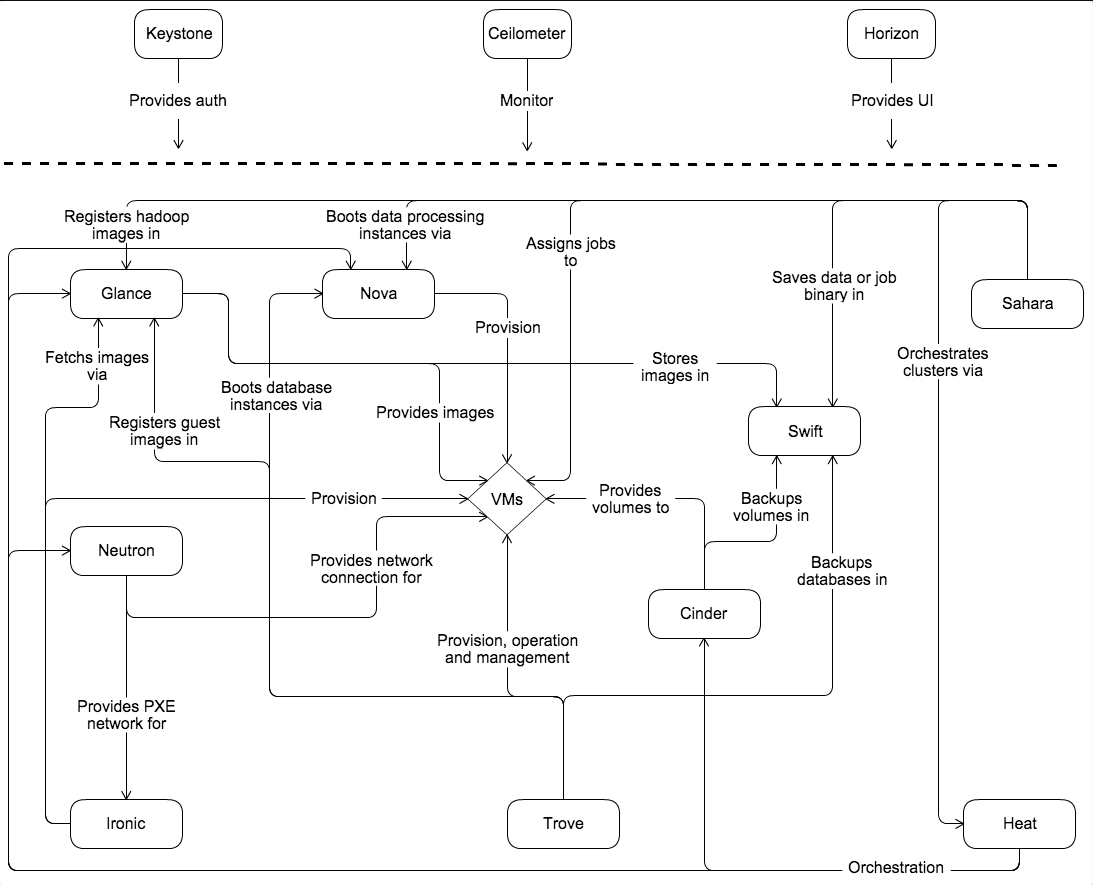
\includegraphics[width=0.8\textwidth]{images/architecture_conceptual_openstack.png}
  \caption*{\textit{Fonte:} \url{https://docs.openstack.org/install-guide/_images/openstack_kilo_conceptual_arch.png}.}
  \label{fig:openstack_conceptual_architecture}
\end{figure}


\section{Componentes do OpenStack}

Discutiremos em mais detalhes como funcionam internamente cada serviços mencionado anteriormente, mostrando como ele interage com o OpenStack de forma geral e suas principais responsabilidades. Focaremos neles porque eles serão essenciais na aplicação para a criação de um cluster.


\subsection{Nova (Compute)}

O \textbf{Nova} é o serviço de computação do OpenStack, responsável por gerenciar o ciclo de vida das instâncias de máquinas virtuais (VMs) e contêineres. Atuando como o motor de computação na nuvem, ele permite que os usuários provisionem e escalem recursos de maneira eficiente. Para provisionar uma instância funcional e acessível, o Nova interage com outros serviços do OpenStack, como Glance, Neutron, Keystone e Placement.

As principais funcionalidades do Nova incluem:

\begin{itemize}
    \item \textbf{Provisionamento de Instâncias:} Criação de instâncias de VMs com diferentes configurações de CPU, memória e armazenamento, atendendo a diversas necessidades de computação.
    \item \textbf{Suporte a Contêineres:} Execução de contêineres, proporcionando uma camada adicional de flexibilidade e eficiência.
    \item \textbf{Escalabilidade:} Administração de grandes quantidades de instâncias, distribuídas em diversos hosts e regiões, com alta escalabilidade.
    \item \textbf{Integração com Outros Componentes:} Interação transparente com serviços como Neutron para gerenciamento de rede e Cinder para armazenamento em blocos, garantindo alocação coordenada e eficiente dos recursos.
\end{itemize}

\subsection{Arquitetura do Nova}

A arquitetura do Nova é composta por vários subcomponentes que colaboram para gerenciar o ciclo de vida das instâncias~\citep{OpenStackNovaArchitecture}. Os principais subcomponentes incluem:

\begin{itemize}
    \item \textbf{nova-api:} Recebe as requisições dos usuários (via API ou Dashboard) e encaminha-as para os demais subcomponentes.
    \item \textbf{nova-scheduler:} Decide em qual nó de computação a instância será criada, consultando o serviço Placement para verificar a disponibilidade de recursos.
    \item \textbf{nova-conductor:} Atua como intermediário entre o nova-compute e o banco de dados, ajudando a minimizar a carga nos nós de computação.
    \item \textbf{nova-compute:} Gerencia a criação, modificação e destruição das instâncias em um nó de computação, interagindo com o \textit{hypervisor} para executar as operações necessárias.
    \item \textbf{nova-placement:} Mantém informações sobre os recursos disponíveis e utilizados no cluster, auxiliando o nova-scheduler na tomada de decisões.
\end{itemize}


\begin{figure}[htbp]
  \centering
  \caption{Estrutura do Nova. A figura mostra os principais subcomponentes do serviço Nova, incluindo \textit{nova-api}, \textit{nova-scheduler}, \textit{nova-conductor}, \textit{nova-compute} e \textit{nova-placement}, e como eles interagem para gerenciar o ciclo de vida das instâncias.}
  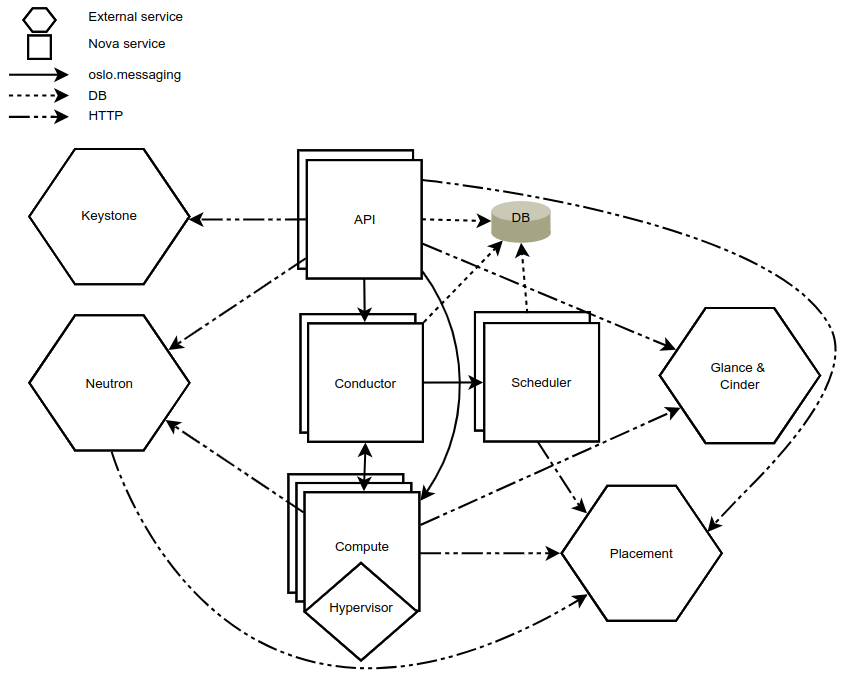
\includegraphics[width=0.7\textwidth]{images/nova_structure.png}
  \caption*{\textit{Fonte:} \citep{DocumentacaoOpenstack}.}
  \label{fig:nova_structure}
\end{figure}


O processo de criação de uma instância no Nova segue estas etapas:

\begin{enumerate}
    \item \textbf{Recepção da Requisição:} O usuário envia uma solicitação para criar uma nova instância através da API do OpenStack.
    \item \textbf{Processamento Inicial:} O \textbf{nova-api} recebe a requisição, cria uma entrada no banco de dados e a coloca em uma fila para processamento pelo \textbf{nova-scheduler} (utilizando o RabbitMQ, um serviço popular de mensageria).
    \item \textbf{Escolha do Nó de Computação:} O \textbf{nova-scheduler} lê a requisição da fila, consulta o \textbf{nova-placement} para verificar a disponibilidade de recursos e seleciona o nó mais adequado aplicando filtros e políticas.
    \item \textbf{Intermediação do Conductor:} O \textbf{nova-conductor} envia as instruções necessárias ao \textbf{nova-compute} do nó selecionado.
    \item \textbf{Interação com o \textit{hypervisor}:} O \textbf{nova-compute} se comunica com o \textit{hypervisor} (como QEMU-KVM) para criar a instância, configurando a rede via Neutron e anexando volumes de armazenamento via Cinder, se necessário.
    \item \textbf{Inicialização da Instância:} Após a criação, a instância é iniciada, e o \textbf{nova-compute} atualiza o estado da instância no banco de dados.
\end{enumerate}


Na escolha do nó de computação, o \textbf{nova-scheduler} aplica diversos filtros para garantir a alocação eficiente das instâncias. Alguns dos principais filtros incluem:

\begin{itemize}
    \item \textbf{AggregateIoOpsFilter:} Filtra nós com base na carga de operações de I/O.
    \item \textbf{AggregateNumInstancesFilter:} Limita o número de instâncias por nó.
    \item \textbf{ComputeCapabilitiesFilter:} Avalia as capacidades de computação dos nós.
    \item \textbf{RamFilter:} Verifica a quantidade de memória RAM disponível.
    \item \textbf{DiskFilter:} Considera a disponibilidade de espaço em disco.
\end{itemize}

Além da criação de instâncias, o Nova gerencia outras operações do ciclo de vida, como:

\begin{itemize}
    \item \textbf{Escalabilidade:} Permite a escala horizontal de instâncias, assegurando o crescimento da infraestrutura conforme necessário.
    \item \textbf{Migração:} Suporta a migração de instâncias entre nós de computação para manutenção ou balanceamento de carga.
    \item \textbf{Redimensionamento:} Permite o ajuste de recursos alocados a uma instância existente.
    \item \textbf{Monitoramento e Recuperação:} Monitora o estado das instâncias e realiza ações corretivas em caso de falhas.
\end{itemize}


\subsection{Neutron (Networking)}

O \textbf{Neutron} é o serviço de gerenciamento e criação de rede, responsável por fornecer conectividade como um serviço entre os componentes do ambiente de nuvem. Ele permite que os usuários criem e gerenciem redes virtuais, sub-redes, roteadores, balanceadores de carga, firewalls e outros recursos de rede de maneira programática, garantindo que as instâncias possam se comunicar entre si e com redes externas.

O Neutron oferece uma ampla gama de funcionalidades que permitem a configuração e gerenciamento de redes de forma flexível e escalável:

\begin{itemize}
    \item \textbf{Criação de Redes Virtuais:} Permite a criação de redes virtuais que conectam as instâncias de VMs, proporcionando isolamento entre diferentes grupos de usuários ou projetos.
    \item \textbf{Gerenciamento de Sub-redes:} Facilita a criação de sub-redes dentro das redes virtuais, com suporte para alocação automática de endereços IP (DHCP) e configuração de gateway.
    \item \textbf{Roteamento e NAT:} Suporta a configuração de roteadores para interconectar sub-redes e fornecer acesso externo às instâncias, incluindo suporte para NAT (Network Address Translation).
    \item \textbf{Segurança de Rede:} Inclui a configuração de firewalls e grupos de segurança que controlam o tráfego de entrada e saída da rede, garantindo um ambiente seguro.
    \item \textbf{Balanceamento de Carga:} Oferece serviços de balanceamento de carga para distribuir o tráfego entre múltiplas instâncias, melhorando a disponibilidade e o desempenho dos aplicativos.
\end{itemize}

Assim como o Nova a arquitetura do Neutron é composta por diversos componentes que colaboram para gerenciar a rede em um ambiente OpenStack. Os principais componentes incluem:

\begin{itemize}
    \item \textbf{neutron-server:} Componente central que expõe as APIs do Neutron e orquestra as operações de rede, interagindo com o banco de dados e os agentes de rede.
    \item \textbf{neutron-plugin:} Abstrai a interação com diferentes tecnologias de rede (como Open vSwitch, Linux Bridge, etc.), permitindo que o Neutron seja compatível com uma variedade de backends.
    \item \textbf{neutron-dhcp-agent:} Gerencia os serviços DHCP para as sub-redes, garantindo que as instâncias recebam endereços IP automaticamente.
    \item \textbf{neutron-l3-agent:} Responsável pelo roteamento de tráfego entre sub-redes e entre a rede interna e externa, implementando funcionalidades de roteamento e NAT.
    \item \textbf{neutron-metadata-agent:} Facilita o acesso das instâncias aos metadados necessários para sua configuração, como as chaves SSH ou dados de inicialização.
    \item \textbf{neutron-lbaas-agent:} Gerencia as operações de balanceamento de carga, criando e configurando balanceadores de carga conforme necessário.
\end{itemize}

\begin{figure}[htbp]
  \centering
  \caption{Fluxo de trabalho do Neutron. A figura ilustra os principais componentes do Neutron, como \textit{neutron-server}, agentes de DHCP, L3, metadados e balanceamento de carga, demonstrando como eles colaboram para fornecer serviços de rede em ambientes OpenStack.}
  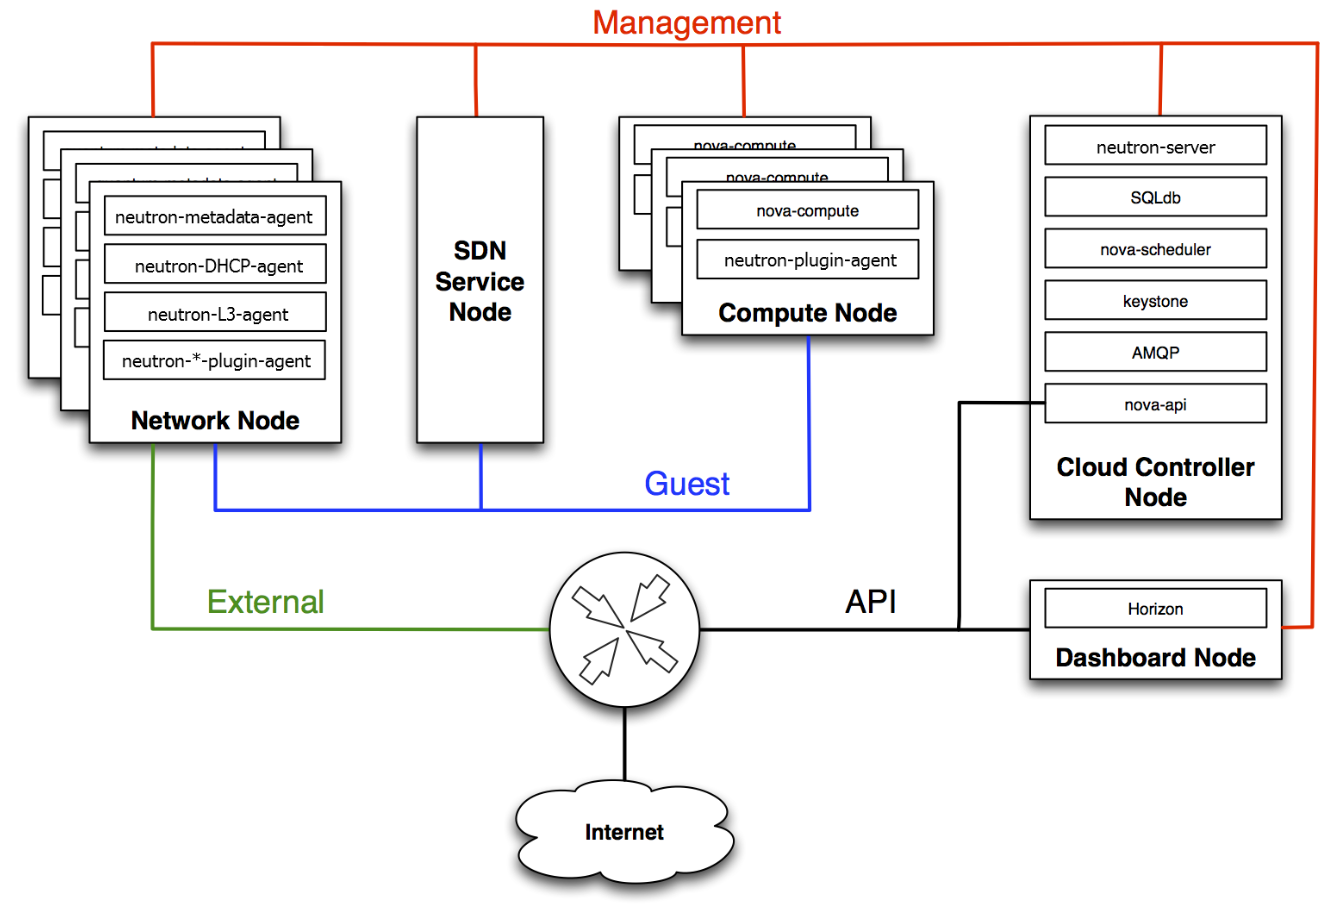
\includegraphics[width=0.8\textwidth]{images/architecture_neutron.png}
  \caption*{\textit{Fonte:} \citep{DocumentacaoOpenstack}.}
  \label{fig:neutron_architecture}
\end{figure}


O processo de criação de uma rede e suas operações no Neutron envolvem várias etapas, que podem ser descritas da seguinte maneira:

\begin{enumerate}
    \item \textbf{Criação de Rede:} O usuário solicita a criação de uma rede virtual via API do Neutron, que é processada pelo \textbf{neutron-server}.
    \item \textbf{Configuração de Sub-rede:} O usuário define uma sub-rede dentro da rede criada, configurando parâmetros como o intervalo de endereços IP, gateway e servidor DHCP.
    \item \textbf{Configuração de Segurança:} O usuário configura grupos de segurança e regras de firewall para controlar o tráfego permitido a conexão para as instâncias conectadas à rede.
    \item \textbf{Roteamento e NAT:} Se necessário, o usuário cria um roteador para interligar sub-redes ou conectar a rede à internet, configurando NAT para que as instâncias possam acessar redes externas.
    \item \textbf{Balanceamento de Carga:} Para distribuir o tráfego entre várias instâncias, o usuário pode configurar um serviço de balanceamento de carga, que será gerenciado pelo \textbf{neutron-lbaas-agent}. Não é necessário criar diretamente um balanceador de carga
\end{enumerate}

A maneira como ela vai ser configurada dentro do OpenStack vai depender totalmente da necessidade do projeto.

\subsection{Keystone (Identity Service)}

O \textbf{Keystone} é o serviço de identidade do OpenStack, responsável por autenticar e autorizar usuários e serviços que interagem dentro da nuvem. Ele desempenha um papel central na segurança e no gerenciamento de acesso, garantindo que apenas usuários e serviços autenticados possam acessar os recursos disponíveis no OpenStack.


O Keystone oferece várias funcionalidades essenciais para a verficação de identidade e controle de acesso:

\begin{itemize}
    \item \textbf{Autenticação e Autorização:} O Keystone valida as credenciais dos usuários e serviços, emitindo tokens que são utilizados para autorizar o acesso aos outros componentes do OpenStack. Esses tokens carregam informações sobre as permissões do usuário ou serviço, garantindo que eles possam acessar apenas os recursos para os quais têm permissão.
    \item \textbf{Gerenciamento de Identidades:} O Keystone gerencia os usuários, grupos, projetos e domínios dentro do OpenStack. Ele permite a criação e atribuição de papéis \textit{(Roles)}, que determinam o nível de acesso e as permissões que cada usuário ou serviço tem dentro de um projeto ou domínio específico.
    \item \textbf{Serviço de Catálogo:} O Keystone mantém um catálogo dos serviços disponíveis no OpenStack, dentro do Horizon podemos ver as respectivas APIs e endpoints. Isso permite que os usuários e serviços descubram e interajam com outros componentes de maneira centralizada e eficiente.
\end{itemize}


O Keystone funciona como uma camada de segurança intermediária que se integra com todos os outros serviços do OpenStack. Quando um usuário ou serviço precisa acessar um recurso, ele primeiro se autentica no Keystone, que verifica as credenciais fornecidas (por exemplo, nome de usuário e senha, ou token). Se a autenticação for bem-sucedida, o Keystone emite um token que o usuário ou serviço pode usar para acessar outros componentes, como Nova, Neutron, ou Glance.

Cada vez que uma solicitação é feita a um serviço do OpenStack, o token é enviado como parte da requisição. O serviço verifica o token com o Keystone para garantir que ele seja válido e que o usuário ou serviço tenha as permissões necessárias para realizar a operação solicitada. Se o token for válido e as permissões forem adequadas, o serviço processa a requisição.

\subsection{Interação KeyStone com outros componentes}
O Keystone é essencial para a operação segura e eficiente de toda a infraestrutura do OpenStack. Todos os serviços, como Nova, Neutron, Glance, Cinder, e Swift, dependem do Keystone para autenticação e autorização. Quando um serviço precisa verificar as permissões de um usuário, ele consulta o Keystone, o que garante que todas as operações dentro do OpenStack estejam protegidas por um controle de acesso robusto ~\citep{da2018self}.

\begin{figure}[htbp]
  \centering
  \caption{Autenticação de serviços e usuários no Keystone. A figura demonstra como o Keystone gerencia a autenticação e autorização de usuários e serviços no OpenStack, emitindo tokens e verificando permissões para garantir acesso seguro aos recursos.}
  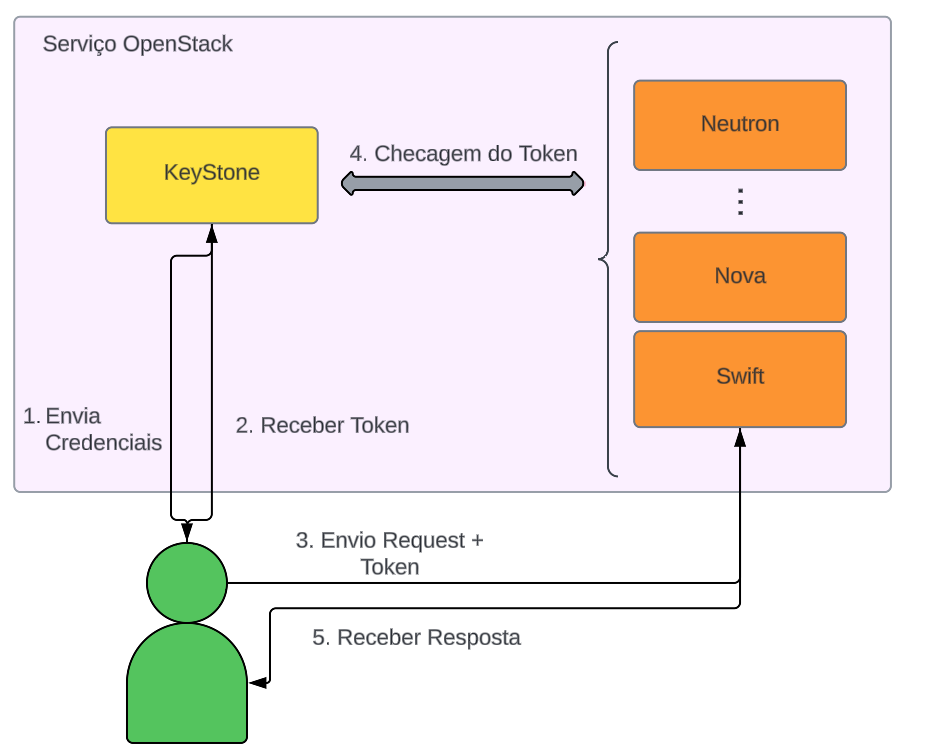
\includegraphics[width=0.7\textwidth]{images/keystone_architecture_2.png}
  \caption*{\textit{Fonte:} Adaptado de~\citep{da2018self}.}
  \label{fig:keystone_architecture}
\end{figure}


Além disso, o catálogo de serviços mantido pelo Keystone é fundamental para que os usuários e serviços descubram quais APIs e endpoints estão disponíveis, facilitando a comunicação e interação dentro do ambiente de nuvem.

Por fim, a capacidade do Keystone de integrar-se com sistemas de autenticação externos, através de federação e SSO, torna-o altamente versátil e adaptável a diferentes ambientes corporativos, garantindo uma experiência de usuário coesa e segura em organizações de todos os tamanhos.

Este papel central do Keystone na segurança e no gerenciamento de acesso faz dele um componente crítico no ecossistema OpenStack, assegurando que apenas usuários e serviços autorizados possam operar dentro da nuvem.


\subsection{Cinder (Block Storage)}

O \textbf{Cinder} é o serviço de armazenamento em bloco, responsável por gerenciar volumes de armazenamento que podem ser anexados a instâncias de máquinas virtuais. Ele fornece uma solução flexível e escalável para armazenar dados de maneira persistente, permitindo que os volumes sejam criados, gerenciados e conectados ou desconectados de instâncias conforme necessário~\citep{rosado2014overview}.

O armazenamento em bloco divide os dados em blocos e os armazena em partes separadas cada um com identificador exclusivo, dentro do sistema cada bloco é tratado como um disco individual, utilizamos dele para dar armazenamento a instância. Essa forma deixa fácil a duplicação do armazenamento para copias ou recuperar dados~\citep{BlockStorage}.

As principais funcionalidades do Cinder incluem:

\begin{itemize}
    \item \textbf{Criação e Gerenciamento de Volumes:} Permite que os usuários criem volumes de armazenamento que podem ser anexados a instâncias para uso como discos adicionais. Esses volumes podem ser criados a partir de imagens, snapshots, ou de forma vazia.
    \item \textbf{Snapshots:} O Cinder suporta a criação de snapshots de volumes, permitindo que os dados sejam salvos em um ponto no tempo para backup ou clonagem futura.
    \item \textbf{Tipos de Armazenamento:} Oferece a possibilidade de definir diferentes tipos de armazenamento, permitindo a escolha entre diversos backends de armazenamento com diferentes características de desempenho e custo.
    \item \textbf{Expansão de Volumes:} Volumes existentes podem ser expandidos conforme necessário, sem a necessidade de desconectar o volume da instância.
    \item \textbf{Conectividade Multi-backend:} Suporta múltiplos backends de armazenamento, como LVM, NFS, Ceph, e outros, proporcionando flexibilidade na escolha do hardware e arquitetura de armazenamento.
\end{itemize}

A arquitetura geral do Cinder se divide em:

\begin{itemize}
    \item \textbf{Cinder-API}: Exposição da interface RESTful para gerenciamento de volumes.
    \item \textbf{Cinder-Scheduler}: Responsável por determinar qual backend de armazenamento deve ser usado para criar um volume.
    \item \textbf{Cinder-Volume}: Gerenciamento direto de volumes nos backends de armazenamento.
    \item \textbf{Cinder-Backup}: Criação e gerenciamento de backups de volumes em armazenamento    secundário.
    \item \textbf{Cinder-Client}: Ferramenta de linha de comando para interagir com a API do Cinder.
\end{itemize}


\begin{figure}[htbp]
  \centering
  \caption{Arquitetura do Cinder. A figura apresenta os principais componentes do serviço Cinder, incluindo \textit{cinder-api}, \textit{cinder-scheduler}, \textit{cinder-volume}, \textit{cinder-backup}, e \textit{cinder-client}, ilustrando como eles colaboram para fornecer armazenamento em bloco persistente e escalável no OpenStack.}
  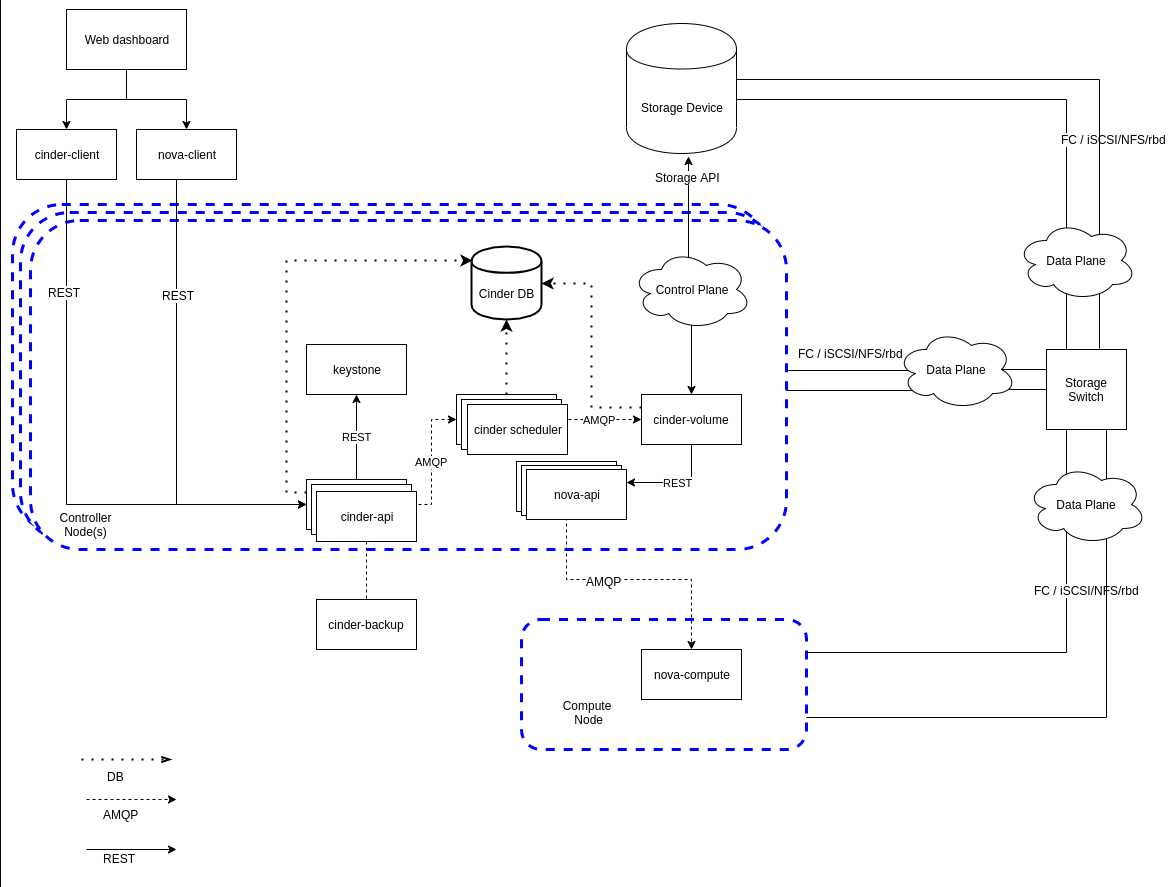
\includegraphics[width=0.95\textwidth]{images/cinder_architecture.png}
  \caption*{\textit{Fonte:}~\citep{OpenStackCinder}.}
  \label{fig:cinder_architecture}
\end{figure}


O Cinder é crucial para aplicações que exigem armazenamento de dados persistente e de alto desempenho, como bancos de dados e sistemas de arquivos distribuídos. Sua capacidade de integrar-se com diversos tipos de armazenamento e fornecer snapshots e backups automáticos torna-o um componente vital para a infraestrutura de nuvem do OpenStack por se ligar as instâncias~\citep{OpenStackCinder}.


\subsection{Swift (Object Storage)}

O \textbf{Swift} é o serviço de armazenamento de objetos, projetado para armazenar e recuperar grandes volumes de dados não estruturados de forma escalável e redundante. Diferente do armazenamento em bloco, o Swift armazena dados como objetos, que são agrupados em contêineres e acessados via uma API RESTful, sem a necessidade de gerenciar um sistema de arquivos tradicional ~\citep{OpenStackSwitft}, segue a mesma ideia do \textit{S3 AWS}, assim você consegue salvar todos os arquivos e acessar eles pelo ID de forma eficiênte via API.

O armazenamento de objetos encapsula dados em unidades chamadas objetos, que incluem tanto os dados quanto seus metadados e atributos. Essa abordagem permite um gerenciamento mais flexível e escalável dos dados, distribuindo a carga de trabalho entre dispositivos de armazenamento inteligentes, conhecidos como \textit{Object-based Storage Devices (OSDs)}, que oferecem alta performance e segurança em ambientes de computação distribuída"~\citep{panasas2007object}.

As principais funcionalidades do Swift incluem:

\begin{itemize}
    \item \textbf{Armazenamento Escalável de Objetos:} Permite armazenar uma quantidade ilimitada de dados distribuídos entre múltiplos servidores, garantindo escalabilidade horizontal.
    \item \textbf{Redundância e Replicação:} Implementa replicação automática dos dados para assegurar alta disponibilidade e durabilidade, mesmo em caso de falhas de hardware.
    \item \textbf{Acesso via API RESTful:} Os dados podem ser acessados e gerenciados através de uma API RESTful, facilitando a integração com aplicações e serviços web.
    \item \textbf{Gerenciamento de Contêineres:} Organiza os objetos em contêineres, permitindo que os usuários agrupem dados logicamente e definam políticas de acesso específicas.
    \item \textbf{Versionamento e Auditoria:} Suporta versionamento de objetos e auditoria de acessos, garantindo controle sobre as mudanças e acesso aos dados.
\end{itemize}

O Swift é ideal para armazenar grandes quantidades de dados não estruturados, como backups, arquivos multimídia, e logs. Sua arquitetura distribuída e resiliente o torna uma escolha popular para ambientes que exigem armazenamento de longa duração e alta disponibilidade.

\subsection{Glance \textit{(Image Service)}}

O \textbf{Glance} é o serviço de gerenciamento de imagens, projetado para armazenar, descobrir e recuperar imagens de disco de máquinas virtuais. Ele permite que os usuários façam upload de imagens de sistemas operacionais e outros discos, que podem ser usados para instanciar novas máquinas virtuais. As imagens podem ser armazenadas em uma variedade de backends, como Swift, Ceph, ou em sistemas de arquivos locais.

As principais funcionalidades do Glance incluem:

\begin{itemize}
    \item \textbf{Gerenciamento de Imagens:} Facilita o upload, armazenamento e compartilhamento de imagens de disco, que podem ser usadas para criar novas instâncias de VMs.
    \item \textbf{Conversão de Formatos:} Glance pode converter imagens entre diferentes formatos de disco, proporcionando maior compatibilidade e flexibilidade na utilização das imagens.
\end{itemize}

O Glance é essencial para o provisionamento de instâncias no OpenStack, permitindo que as imagens de sistemas operacionais e discos sejam gerenciadas de forma centralizada e eficiente. Sua integração com outros componentes do OpenStack, como Nova e Cinder, torna-o um elemento crucial para a operação e escalabilidade da nuvem.

\subsection{Heat \textit{(Infraestructure as Code)}}

O \textbf{Heat} é o serviço de orquestração de recursos, projetado para permitir o gerenciamento automatizado e coordenado de infraestruturas complexas. Utilizando templates escritos em YAML, o Heat facilita a criação e o gerenciamento de pilhas de recursos, como instâncias de computação, volumes de armazenamento, redes e outros serviços do OpenStack, de forma declarativa e repetível~\citep{OpenStackHeat}.

O Heat permite que orquestremos toda a infraestrutura de uma organização específica com templates, aceita também o Terraform e o CloudFormation, dois serviços famosos de IaC, a ideia de utilizar esses templates é basicamente configurar um ambiente e não precisar ficar refazendo ele caso necessário, você tem todo controle no template e sabe exatamente quais passos foram feitos para construção ou alocação de determinado recurso.

As principais funcionalidades do Heat incluem:

\begin{itemize}
    \item \textbf{Orquestração de Pilhas de Recursos:} Gerencia a criação, atualização e exclusão de conjuntos de recursos interdependentes como uma única unidade, chamada de pilha (\textit{stack}).
    \item \textbf{Infraestrutura como Código:} Os usuários podem definir a infraestrutura em templates YAML, que descrevem os recursos e as relações entre eles, permitindo a automação de operações e a reprodutibilidade dos ambientes.
    \item \textbf{Automação de Provisionamento:} Suporta a automação de tarefas repetitivas e complexas, como o escalonamento de instâncias de computação e o provisionamento de redes e volumes.
    \item \textbf{Suporte a Vários Templates:} Além dos templates nativos do Heat (HOT - Heat Orchestration Template), também suporta templates no formato AWS CloudFormation, proporcionando flexibilidade na definição dos recursos.
\end{itemize}


\href{https://docs.openstack.org/heat/latest/developing_guides/architecture.html}{Arquitetura geral Heat}:

\begin{itemize}
    \item \textbf{Heat-engine:} É o componente central responsável pelo gerenciamento das pilhas de recursos (\textit{stacks}). O Heat Engine interpreta os templates, cria e gerencia os recursos descritos nos templates, e lida com as operações de ciclo de vida das pilhas, como criação, atualização e exclusão.
    \item \textbf{Heat-api:} Fornece uma interface RESTful que permite aos usuários interagir com o serviço Heat. Através da Heat API, os usuários podem enviar templates, criar e gerenciar pilhas, e consultar o estado das pilhas e recursos.
    \item \textbf{Heat-api-cfn:} Implementa uma API compatível com AWS CloudFormation, permitindo que os usuários usem templates no formato AWS CloudFormation para definir e gerenciar seus recursos. Isso oferece uma compatibilidade adicional para aqueles que estão familiarizados com a infraestrutura como código.
    \item \textbf{Python-heatclient:} É a ferramenta de linha de comando que permite interagir com o serviço Heat. Os usuários podem usar o Heat Client para executar comandos que criam, atualizam, deletam e listam pilhas e recursos no OpenStack.
\end{itemize}


O Heat é ideal para automatizar a implementação e o gerenciamento de infraestruturas complexas e repetitivas em ambientes de nuvem, garantindo consistência, escalabilidade e eficiência operacionais. Sua capacidade de orquestrar diversos serviços do OpenStack em conjunto torna-o uma ferramenta essencial para DevOps e equipes de operações que buscam simplificar a gestão de infraestrutura na nuvem.


\subsection{Trove (Database as a Service)}

O \textbf{Trove} é o serviço de banco de dados como serviço (DBaaS) do OpenStack, projetado para simplificar o gerenciamento e a operação de bancos de dados relacionais e não relacionais em ambientes de nuvem. O Trove permite aos usuários provisionar, configurar, operar e escalar instâncias de banco de dados com facilidade, utilizando uma interface unificada e integrada ao ecossistema OpenStack~\citep1{OpenStackTrove}.

O Trove possibilita o gerenciamento de múltiplos bancos de dados através de uma API RESTful, oferecendo suporte para diversos tipos de bancos de dados, como MySQL, PostgreSQL, MongoDB, entre outros. Isso permite que as organizações mantenham uma infraestrutura de banco de dados flexível e escalável, sem a complexidade tradicional associada à administração de bancos de dados em larga escala.

As principais funcionalidades do Trove incluem:

\begin{itemize}
    \item \textbf{Provisionamento Automatizado de Bancos de Dados:} Facilita a criação de instâncias de banco de dados de forma automatizada, permitindo o provisionamento rápido e eficiente de bancos de dados para diferentes aplicações.
    \item \textbf{Gestão Simplificada:} Oferece ferramentas para gerenciar facilmente backups, restaurações, atualizações de software e monitoramento de desempenho, simplificando a administração de bancos de dados.
    \item \textbf{Suporte a Múltiplos Motores de Banco de Dados:} O Trove suporta uma variedade de motores de banco de dados, tanto relacionais quanto não relacionais, proporcionando flexibilidade para diferentes necessidades de aplicação.
    \item \textbf{Escalabilidade:} Permite a escalabilidade vertical e horizontal das instâncias de banco de dados, garantindo que os recursos possam ser ajustados conforme a demanda aumenta.
\end{itemize}

\href{https://docs.openstack.org/trove/latest/contributor/design.html}{Arquitetura geral do Trove}:

\begin{itemize}
    \item \textbf{Trove-taskmanager:} Responsável por gerenciar as operações assíncronas no Trove, como a criação de instâncias, backups e restaurações. Ele coordena essas tarefas em segundo plano para garantir que sejam executadas de forma eficiente.
    \item \textbf{Trove-api:} Fornece a interface RESTful através da qual os usuários podem interagir com o serviço Trove. Através da Trove API, os usuários podem criar, configurar e gerenciar instâncias de banco de dados.
    \item \textbf{Trove-conductor:} Atua como um intermediário entre o Trove-taskmanager e o banco de dados de controle do OpenStack, garantindo a integridade e a sincronização dos dados de gerenciamento.
    \item \textbf{Trove-guestagent:} Instalado dentro de cada instância de banco de dados provisionada pelo Trove, o Trove-guestagent é responsável por executar as operações específicas do banco de dados, como backups, restaurações e mudanças de configuração, comunicando-se com o Trove-taskmanager para realizar essas tarefas.
    \item \textbf{Python-troveclient:} É a ferramenta de linha de comando que permite aos usuários interagir diretamente com o serviço Trove. O Trove Client permite a execução de comandos para criar, gerenciar e excluir instâncias de banco de dados.
\end{itemize}

O Trove é ideal para organizações que desejam simplificar o gerenciamento de bancos de dados na nuvem, permitindo uma administração eficiente e escalável. Com o Trove, as equipes de operações podem automatizar o provisionamento e a manutenção de bancos de dados, garantindo um desempenho consistente e reduzindo a complexidade operacional.


\subsection{Recapitulando}

Como vimos, o OpenStack é composto por diversos componentes que interagem entre si para formar uma infraestrutura como serviço (IaaS) robusta e escalável. Exploramos em detalhe alguns dos componentes mais importantes, como Nova, Neutron e Keystone, que são fundamentais para o funcionamento do OpenStack e serão amplamente utilizados na implementação do nosso projeto.

O OpenStack continua a evoluir, ganhando popularidade e recebendo novas funcionalidades a cada ano. Por essa razão, a análise dos componentes foi abordada de forma geral, destacando aspectos arquiteturais e operacionais essenciais. É importante ressaltar que, embora tenhamos focado nos componentes mais amplamente utilizados, o OpenStack oferece uma gama ainda maior de serviços que podem ser personalizados para atender a necessidades específicas.


\section{Orquestração de VMs}

A orquestração de VMs torna-se essencial em ambientes onde a quantidade de instâncias supera a capacidade de gerenciamento manual. Inicialmente, quando lidamos com poucas instâncias, o uso de um \textit{hypervisor} para controlar as máquinas virtuais pode ser suficiente. Um \textit{Virtual Machine Monitor (VMM)} pode monitorar logs, verificar o uso de recursos e reiniciar instâncias quando necessário. Entretanto, à medida que a infraestrutura se expande, o gerenciamento de dezenas ou centenas de VMs se torna inviável sem uma camada de orquestração.

Aqui entra o OpenStack, que proporciona uma plataforma escalável e flexível para gerenciar grandes quantidades de recursos computacionais. Ele automatiza tarefas como a criação de novas instâncias, a distribuição de recursos entre elas, e a recuperação de falhas, tudo isso através de uma interface centralizada. Para ilustrar, enquanto uma pequena empresa poderia gerenciar manualmente poucas instâncias, uma grande organização com picos de demanda e infraestrutura complexa, como uma empresa de e-commerce de grande porte, exigiria orquestração automática para manter a continuidade do serviço em momentos de alta carga, como em eventos sazonais.

A orquestração de VMs não se resume apenas à criação e destruição de instâncias, mas envolve uma série de processos automatizados, como provisionamento, escalabilidade automática, e monitoramento contínuo. Esses processos garantem que a infraestrutura esteja sempre otimizada e pronta para atender às demandas crescentes, minimizando o tempo de inatividade e maximizando a eficiência dos recursos.

\section{Orquestração de Containers}

A orquestração de containers segue uma lógica semelhante à de VMs, porém com um nível de granularidade e agilidade muito maior. Containers são instâncias leves que compartilham o mesmo sistema operacional do host, o que permite que sejam inicializados rapidamente e consumam menos recursos em comparação com VMs completas. No entanto, com a proliferação de containers em um ambiente de produção, gerenciá-los manualmente também se torna inviável. É aí que entra o Kubernetes, uma das ferramentas mais utilizadas para orquestração de containers.

O Kubernetes permite gerenciar de forma eficiente centenas ou até milhares de containers, distribuindo a carga de trabalho entre diferentes nós e garantindo que os serviços continuem funcionando, mesmo que algum nó falhe. Ele utiliza um sistema baseado em declarações em um arquivo \textit{.yaml}, onde o administrador define o estado desejado da aplicação (quantidade de containers, recursos utilizados, etc.), e o Kubernetes se encarrega de garantir que esse estado seja mantido.

Além disso, o Kubernetes facilita o escalonamento de aplicações, monitorando o desempenho dos containers e adicionando ou removendo instâncias conforme necessário. Isso é particularmente útil em arquiteturas baseadas em microserviços, onde diferentes partes de uma aplicação podem ser escaladas de maneira independente, melhorando a eficiência e o uso de recursos~\citep{KubernetsDocumentation}.

\subsection{Estrutura do Kubernetes}

O Kubernetes é composto por vários componentes que, juntos, formam um sistema robusto de orquestração como podemos ver na figura \ref{fig:structure_kubernets}. Os principais elementos da arquitetura do Kubernetes incluem:


\begin{figure}[htbp]
  \centering
  \caption{Estrutura do Kubernetes. A figura apresenta os principais componentes do Kubernetes, como nós, pods, plano de controle (\textit{Control Plane}), \textit{Scheduler}, \textit{Kubelet} e serviços, ilustrando como eles interagem para orquestrar aplicações distribuídas de forma eficiente.}
  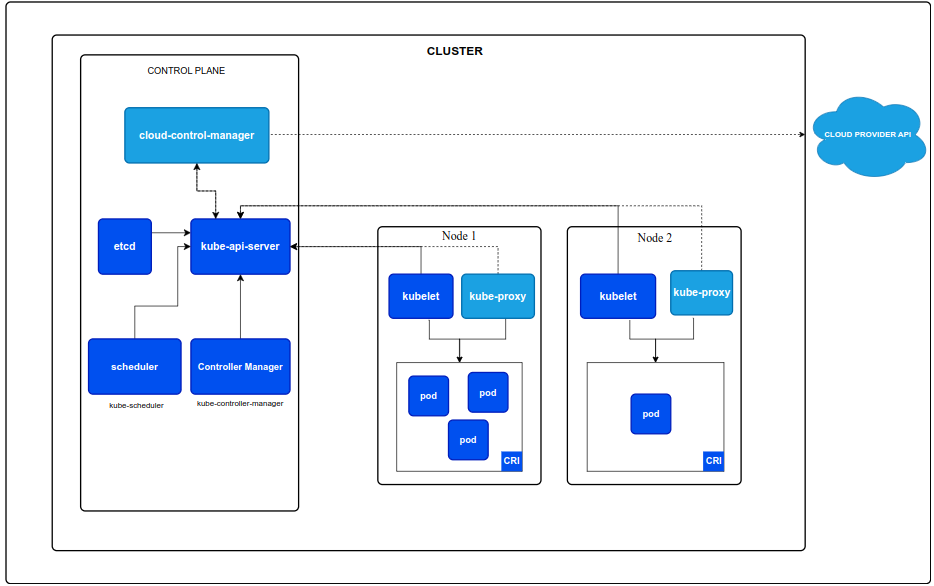
\includegraphics[width=0.9\textwidth]{images/structure_kubernets.png}
  \caption*{\textit{Fonte:} \url{https://kubernetes.io/docs/concepts/architecture/}.}
  \label{fig:structure_kubernets}
\end{figure}


\begin{itemize}
    \item \textbf{Nó (Node):} Cada máquina física ou virtual dentro do cluster do Kubernetes é chamada de nó. Um nó pode conter um ou mais containers.
    \item \textbf{Pods:} O pod é a menor unidade de execução no Kubernetes e pode conter um ou mais containers. Todos os containers dentro de um pod compartilham o mesmo endereço IP e espaço de rede, por padrão cada pod possui apenas um container.
    \item \textbf{Control Plane:} A camada de controle central que gerencia os nós do cluster e garante que o estado desejado das aplicações seja mantido.
    \item \textbf{Scheduler:} Responsável por alocar pods nos nós disponíveis de acordo com os requisitos de recursos e políticas definidas.
    \item \textbf{Kubelet:} Um agente que roda em cada nó do cluster e garante que os containers estejam executando conforme o especificado pelo Kubernetes.
    \item \textbf{Service:} Um serviço que expõe um conjunto de pods como uma única entidade, facilitando o balanceamento de carga e a descoberta de serviços.
\end{itemize}

Com essa arquitetura, o Kubernetes permite que as empresas implementem e gerenciem aplicações distribuídas de forma eficiente, garantindo alta disponibilidade, resiliência e facilidade de manutenção. Também pode ser feita a integração a nossa nuvem privada utilizando o componente Magnum do OpenStack.

